\chapter{Fejlesztői dokumentáció}
\label{ch:impl}

\section{Technológiai stack kiválasztása}

A rendszer technológiai környezetének kiválasztásában fontos szerepet játszott a már meglévő nyelvelemző eszközök elérhetősége, gyors és egyszerű fejlesztés lehetősége, és hogy fejlesztőként ne kevésbé ismert, nehezen bővíthető és karbantartható eszközöket használjunk.

\subsection{Fejlesztői környezet}

A fejlesztés a \textit{Visual Studio Code} nyílt forráskódú kódszerkesztőben történt. A soknyelvű integrációja, beépített Git verziókezelése, kiegészítők támogatása miatt volt ideális választás. A projekt a Python 3.11 vagy újabb verziókra és Django ökoszisztémára épül, a nyelv könnyen tanulhatósága, gyakori használata és sok hasznos NLP és egyéb könyvtár elérhetősége miatt. A függőség- és csomagkezelés megkönnyítésének érdekében \texttt{virtualenv} virtuális környezetben történt a fejlesztés. A verziókezelés Git és GitHub segítségével történt, a \texttt{CI/CD} folyamatokkal együtt, ideértve a tesztfuttatást és a \texttt{flake8} alapú lint-ellenőrzéseket is. 

\subsection{Frontend keretrendszer}

A kliensoldali réteg kialakításánál is fontos szempont volt az egyszerűség, és a már meglévő integráció felhasználása, így a Django beépített template rendszerének használatára esett a választás. Ezen felül keretrendszer REST API integrációja megkönnyítette az objektumok listáihoz és nézeteihez tartozó oldalak kreálását, jelentősen csökkentve a fejlesztési időt és a hibalehetősége számát is. A rendszer a felhasználói élmény fokozása érdekében a HTML sablonokhoz előre megtervezett komponenseket alkalmaz TailWind CSS és DaisyUI segítségével, hogy egyszerűbb és harmonikusabb UI-élményt, valamint egységes és letisztult kinézetet nyújtson. 

A projektben bizonyos esetekben JavaScript használatára is szükség volt (modál ablakok, AJAX interakciók, egyes dinamikus listák frissítése). Ezek a fájlok külön szerepkörökre bontva, csak a szükséges oldalakon kerülnek betöltésre, csökkentve a frontend komplexitását.

Alternatívaként felmerült a fejlesztés elején React vagy Angular használata, de a projekt mérete valamint a keretrendszer által biztosított alternatívánál jelentősen nagyobb komplexitás ezt nem indokolta.

\subsection{Backend keretrendszer}

A backend a Django, egy webes alkalmazásokra specializálódott nyílt forráskódú keretrendszerre épült. Fontos szempont volt a kiválasztásánál a Python nyelven történő fejlesztés és bővíthető admin felület, amelyek elősegítik az adatok gyorsabb elérését és nyomon követését fejlesztés közben is. Továbbá nélkülözhetetlen volt a beépített ORM (Object-Relational Mapping), ami a gyors adatkezelési folyamatokat biztosít mint például kapcsolatkezelés (például Many-to-many kapcsolatok szó és kanji objektumok között), automatikus indexelések a szűrésekhez és keresésekhez. REST API integrációja miatt a kliensoldali megjelenítés is akadálymentesen történik, csökkentve a frontend fejlesztéséhez szükséges munka komplexitását is. Moduláris felépítése miatt ideális és ajánlott is a projektet különböző appokra szétbontani felelősségek és funkcionalitások szerint, ami szinten megegyezett a szoftver tervezett irányelvével.

A fejlesztés megkezdése előtt több keretrendszer használata is felmerült, mint például a Laravel, vagy más Swagger UI-t használó alternatívák mint a Django Ninja és FastAPI. De végül a Python kompatibilitás, integrált ORM és, admin felületek miatt a Django volt az egyértelmű választás.

\subsection{Adatbázis}

Az adatok tárolására és kezelésére SQLite adatbázist alkalmazunk. Fejlesztés közben fontos szempont volt az egyszerű beállíthatóság, ne legyen szükség külön szerverre az adatbázis futtatásához és hogy az ehhez hasonló kis- vagy közepes méretű projektekhez ideális legyen.

Bár kezdetben tervben volt a PostgreSQL-re váltás a fejlesztés végére, de a rendszer jelenlegi funkciói és mérete nem indokolja egy komplexebb, szerver alapú adatbázis bevezetését. Természetesen ha a projekt nagysága, felhasználói köre vagy funkcionális igényei a jövőben jelentősen növekednének, a Django keretrendszer egyszerű áttérési lehetőséget biztosít egy másik adattárolási rendszerre az adatbázisban tárolt adatok megtartásával, és nem szükséges nagymértékű kódmódosítás.

\subsection{NLP modulok és külső könyvtárak}

A nyelvi feldolgozáshoz több külső Python könyvtár integrálására volt szükség. A japán nyelvű tokenizálást a MeCab könyvtár végzi a \texttt{unidic-lite} szótár segítségével, amelyek ezen a területen az ipari standardnak számítanak. Angol nyelven a \texttt{spaCy}-t alkalmazzuk, bár itt több lehetőség közül is lehetett választani. Alternatívaként a \texttt{Stanza} is kipróbálásra került, de az inkább kisebb volumenű projektekhez tervezett és ezáltal gyorsabban elemző spaCy jobban megfelelt fejlesztői igényeknek. Az adatbázisban nem szereplő angol szavak fordítására a \texttt{Deep Translate} könyvtárt vettük igénybe, amely ingyenes használatba vétel esetén csak korlátozott számú kérést engedélyez. Azonban csak az eddig tokenizálatlan elemeken hajtódik végre ez a folyamat, így ennek a limitnek az átlépése nem valószínű a program jelenlegi állapotában.

Az adatok exportálásához az \texttt{openpyxl} (Excel) és a beépített \texttt{csv} modult használjuk. Ezek a könyvtárak a mind jól integrálhatók és széles körben használtak.

A kód minőségéért és egységességének megőrzéséért a formázására \texttt{black}, míg a komplexitás és stílusellenőrzésre \texttt{flake8} fejlesztői eszközöket használtunk.

Több egyéb csomag is szerepel a projektben (pl. \texttt{asgiref}, \texttt{sqlparse}, \texttt{packaging}), ezek főleg a Django vagy egyéb fejlesztői eszközök függőségei, amelyek automatikusan szükségesek a rendszer működéséhez.

\section{A program áttekintése}

A LanDB projekt architektúrája a klasszikus háromrétegű webes alkalmazások mintáját követi, amelyben a frontend (kliensoldali felület), backend (szerveroldali logika) és a perzisztenciáért felelős adatbázis rétegek egymástól elkülönülve hajtják végre respektív feladataikat. Ez növeli a rendszer karbantarthatóságát, átláthatóbba teszi azt és letisztultabb, egyszerűbb lehetőséget biztosít a későbbi bővítésre, vagy akár a technológiai stack egyes elemeinek lecserélésre is. A rétegek közötti kommunikációt a \ref{fig:layers}.~ábra mutatja be:

\begin{figure}[H]
	\centering
	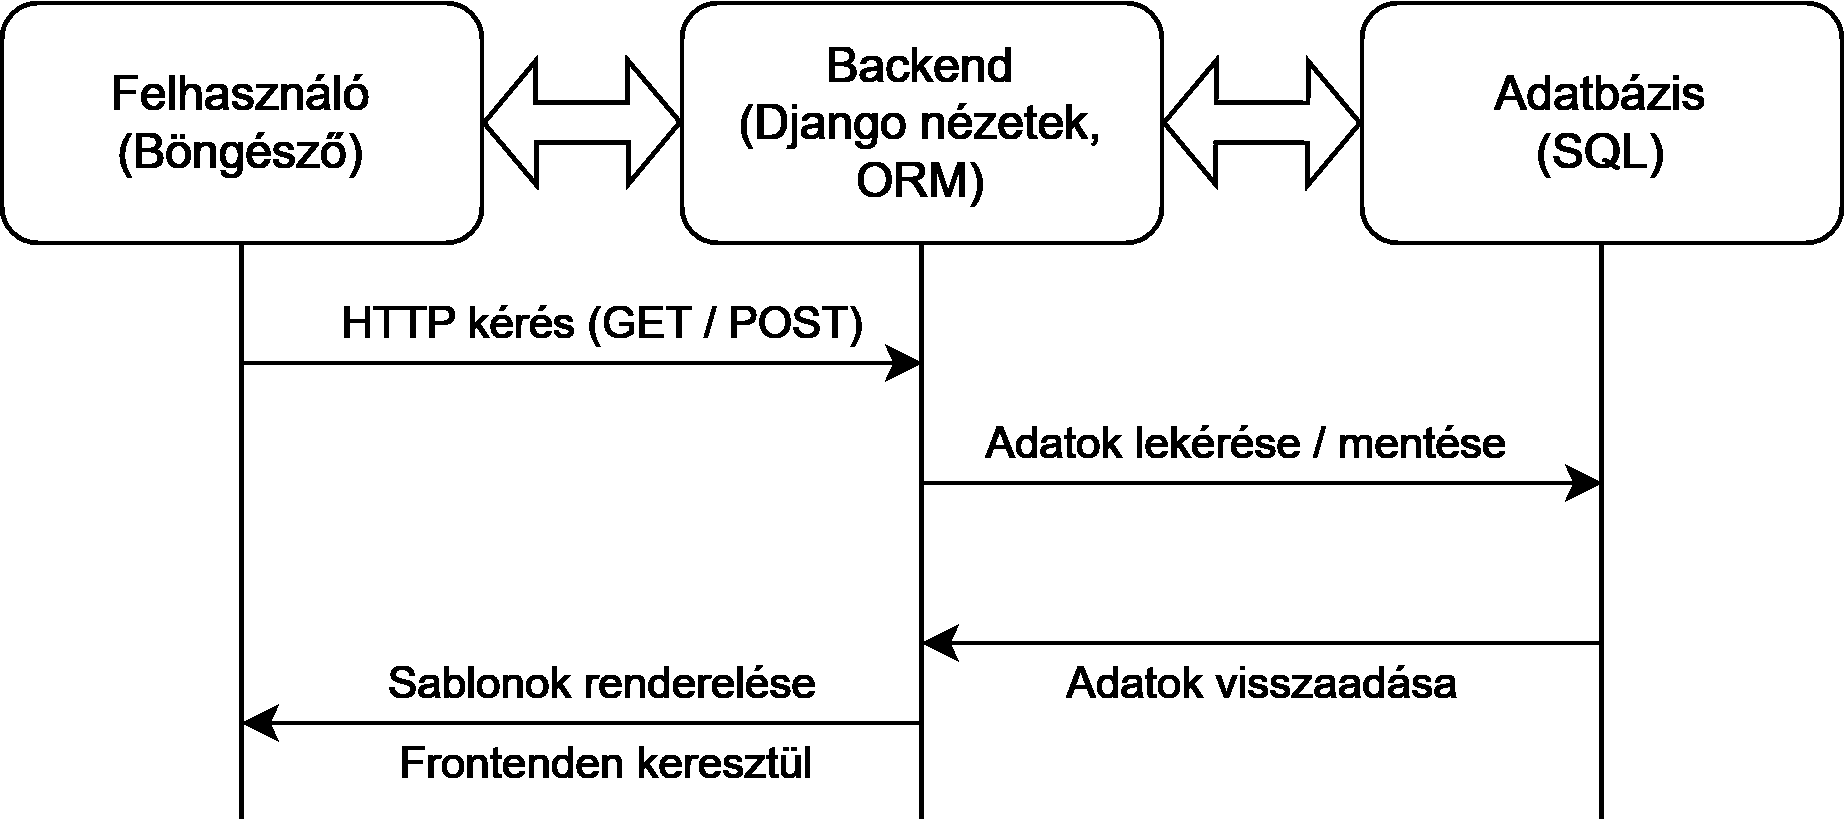
\includegraphics[width=1\textwidth]{images/impl/layers.png}
	\caption{A háromrétegű architektúra működése}
	\label{fig:layers}
\end{figure}

\subsection{Rendszer rétegei}

\subsubsection{Frontend réteg}

Az alkalmazás frontend, más néven kliensoldali rétege felelős a felhasználói felület megjelenítéséért valamint a felhasználó és a rendszer közötti interakciók kezeléséért. Ez a réteg biztosítja, hogy a backend által előállított adatok áttekinthető, logikus és esztétikus formában jelenjenek meg a felhasználó számára. A frontend teljes egészében a Django beépített template rendszerére épül a szerveroldali renderelés elvét követve, amely lehetővé teszi a háttérrendszer által készített anyagokból történő HTML generálást. Ez azt jelenti, hogy a backend nézetek (\textit{views}) által előállított adatok egy \textit{context} formájában kerülnek átadásra a sablonoknak, amelyekből dinamikusan készül el a végső HTML oldal.

A frontend réteg architekturális szempontból a backend és a felhasználó között helyezkedik el. Minden felhasználói művelet (például keresés, szűrés, tanulási statisztikák megtekintése) egy HTTP-kérésen keresztül jut el a szerverhez, amely feldolgozza azt, majd a válaszként kapott adatok itt kerülnek megjelenítésre. A rendszer alapvetően szerveroldali \textit{renderelésre} épül, így a kliensoldali logika minimális, a fő hangsúly a sablonokban történő adatmegjelenítésen van. 

Az általános felhasználói élmény javítása érdekében a projektben helyenként aszinkron kommunikáció is megjelenik, például egyes elemek, mint a tanulási kártyák gyors frissítése, vagy bizonyos felhasználói beállításokat kezelő ablakok megjelenítése és bezárása AJAX segítségével kerültek megvalósításra. A rendszer alapvető funkciói és műveletei megfelelő működése azonban JavaScript támogatás hiányában is teljes mértékben biztosított.

Összességében a LanDB alkalmazás architektúrájában a frontend a backend és felhasználó közötti közvetítő szerepét tölti be, biztosítva az adatok helyes vizuális megjelenítését valamint a backend funkciók egyszerű elérését. A konkrét sablonok, komponensek és kódszerkezet részletes bemutatására a későbbi \ref{moduls} fejezetben fog sor kerülni.

\subsubsection{Backend réteg}

A LanDB alkalmazás backend rétege architekturális szempontból a rendszer központi eleme, amely egybefogja a különböző funkciókat, és biztosítja ezek egységes működését. Ez felelős az üzleti logika megvalósításáért, az adatkezelésért, valamint a felhasználói kérések feldolgozásáért. Ez a réteg közvetít a frontend felület és az adatbázis között, biztosítva, hogy a felhasználó által kezdeményezett műveletek (például szűrés, keresés, tanulási statisztikák lekérdezése, szótárak kezelése) megfelelően végrehajtódjanak, és az eredmények helyesen jussanak vissza. 

Fogadja a frontend rétegtől érkező HTTP-kéréseket, majd ezek alapján a \texttt{request} feldolgozása után lekéri, módosítja vagy eltávolítja a megfelelő elemeket. Ezeket a folyamatokat a Django ORM biztosítja adatbázis műveleteken keresztül, így a fejlesztőnek nem kell manuális SQL lekérdezéseket írnia és implementálnia.  Miután az adatok feldolgozásra kerültek, végrehajtódtak az itt történő ellenőrzések, funkciók és számítások, a réteg a kliensoldal felé visszaküld egy \texttt{context} formájú választ amely ezekből generálja a felhasználó által elérhető HTML oldalakat.

A backend réteg felel továbbá a rendszer integritásáért és biztonságáért is. Gondoskodik többek között az adatok validálásáról valamint a hibák megfelelő kezeléséről. A rendszer bővíthetősége és karbantarthatósága szempontjából is kulcsfontosságú, hiszen minden új funkció vagy üzleti logika ebben a rétegben valósul meg, miközben a frontend és az adatbázis réteg változatlanul maradhat.

\subsubsection{Adatbázis}

Az adatbázis réteg képviseli a rendszer alapját, hiszen itt történik meg minden nyelvi egység, tanulási adat és statisztika strukturált tárolása. Ez egy SQLite alapú relációs adatbázis, amelyet a Django ORM kezel, a backend rendszer számára egységes strukturált elérést biztosítva. 

A projektben szereplő nyelvi egységek (szöveg, mondat, szó, kanji) itt jelennek meg külön táblákban definiálva, valamint itt jönnek létre a köztük lévő kapcsolatokat biztosító idegen kulcsú (\texttt{ForeignKey}) vagy több-a-többhöz (\texttt{Many-to-many}) relációk. Ez a szerkezet biztosítja, hogy egy szöveghez több mondat, egy mondathoz több szó, egy szóhoz több kanji vagy kanjihoz több szó is tartozhasson. Ugyanitt kerülnek eltárolásra a tanulási folyamat során generált adatok is, például egy nyelvi elemhez kapcsolódó, dátumhoz kötött válaszok tömbje, amelyek JSON alapú, strukturált mezőkben helyezkednek el, de ezekről részletesebben szó lesz a Modulok, appok és kódszerkezet című, \ref{moduls} fejezetben.

A felhasználó által generált adatokon kívül, itt kerülnek eltárolásra az úgynevezett referencia-objektumok is. Ezek a referencia modellek tartalmazzák a jelenleg támogatott nyelvekhez tartozó egységek lexikális háttéradatait, mint például nyelvvizsga szintek, gyakoriságok vagy japán szavaknál olvasatok, jelentések. Ezek az adatok képzik a nyelvi feldologozás, szótárak összeállítása és tanulási funkciók alapjait. A rendszer első indításakor vagy egy külön parancs futtatásakor ezek a referencia-objektumok előre elkészített, beégetett fájlokból jönnek létre, amelyek a projekt \texttt{data} mappájában találhatók, és automatikusan feltöltődnek az adatbázisba.

Ez az architekturális megközelítés lehetővé teszi, hogy a rendszer egyszerre legyen rugalmas, mivel a felhasználó képes kezelni saját szavait, szövegeit és más nyelvi elemeit, ugyanakkor szakmailag megbízható, hiszen a referencia adatok iparági standard forrásokból származnak amelyek automatikusan és szabadon frissíthetők vagy bővíthetők.

\subsubsection{Rétegek közti kommunikáció}

A rendszer minden komponense a Django által biztosított absztrakciókon keresztül kommunikál, így a rétegek közötti adatcsere egységes, könnyen karbantartható és bővíthető. Oldalak, mint a szavak vagy írásjelek listáját megjelenítő \textit{Words} és \textit{Kanji} menüpontok \texttt{GET} kérések segítségével töltődnek be, valamint az itt elhelyezkedő szűrők által végzett relációs műveletek is így működnek. Adatok módosításakor vagy létrehozásakor a program \texttt{POST} kéréseket használ, így történik többek között a szövegek feltöltése, elemek hozzáadása vagy eltávolítása szótárakból, szövegek letöltése különböző formátumokban vagy tanulás közben a felhasználó válasza után az elem adattagjainak a módosítása.

\subsection{Modulok, appok és kódszerkezet}\label{moduls}

A LanDB projekt kódbázisa a Django ajánlásait követve több alkalmazásra és közös mappára tagolódik. Az alábbiakban áttekintjük a projekt főbb szerkezeti egységeit, hol találhatók a különböző funkciók, modellek, nézetek, segédfüggvények és statikus vagy tartalmi elemek.

\subsubsection{Gyökérkönyvtár}

A projekt gyökérkönyvtára tartalmazza a projekt indításához és adminisztrációjához szükséges szkripteket (\texttt{start.ps1}, \texttt{start.bat}), ezek hozzák létre a szintén itt található virtuális gépet (\texttt{venv} mappa) az első indításakor, ahova a függőségeket tartalmazó \texttt{requirements.txt} segítségével a rendszer helyes működéséhez szükséges csomagok telepítésre kerülnek. Az szkriptek felelnek továbbá az adatbázishoz tartozó migrációk lefutásáért, a referenciaadatok betöltéséért és a szerver elindításáért.

Szintén itt helyezkednek el a verziókezelés működöséhez elengedhetetlen \texttt{.gitignore} és \texttt{README.md}, és a CI/CD folyamat során  használt \texttt{.flake8} (lint ellenőrzéshez) és \texttt{django.yaml} állományok is. A felépítés látható a \ref{fig:folders}.~ábrán.

\begin{figure}[H]
	\centering
	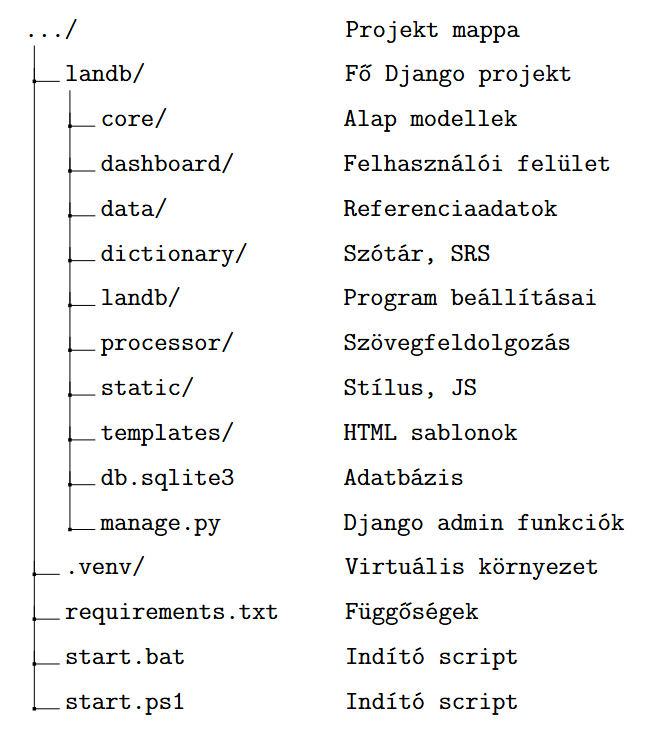
\includegraphics[width=0.75\textwidth]{images/impl/folder_system.png}
	\caption{A gyökérmappa felépítése és fontosabb elemei}
	\label{fig:folders}
\end{figure}

\iffalse
\dirtree{%
.1 \makebox[5cm][l]{.../} \makebox[8cm][l]{Projekt mappa}.
.2 \makebox[4,3255cm][l]{landb/} \makebox[8cm][l]{Fő Django projekt}.
.3 \makebox[3,7255cm][l]{core/} \makebox[8cm][l]{Alap modellek}.
.3 \makebox[3,725cm][l]{dashboard/} \makebox[8cm][l]{Felhasználói felület}.
.3 \makebox[3,725cm][l]{data/} \makebox[8cm][l]{Referenciaadatok}.
.3 \makebox[3,725cm][l]{dictionary/} \makebox[8cm][l]{Szótár, SRS}.
.3 \makebox[3,725cm][l]{landb/} \makebox[8cm][l]{Program beállításai}.
.3 \makebox[3,725cm][l]{processor/} \makebox[8cm][l]{Szövegfeldolgozás}.
.3 \makebox[3,725cm][l]{static/} \makebox[8cm][l]{Stílus, JS}.
.3 \makebox[3,725cm][l]{templates/} \makebox[8cm][l]{HTML sablonok}.
.3 \makebox[3,725cm][l]{db.sqlite3} \makebox[8cm][l]{Adatbázis}.
.3 \makebox[3,725cm][l]{manage.py} \makebox[8cm][l]{Django admin funkciók}.
.2 \makebox[4,325cm][l]{.venv/} \makebox[8cm][l]{Virtuális környezet}.
.2 \makebox[4,325cm][l]{requirements.txt} \makebox[8cm][l]{Függőségek}.
.2 \makebox[4,325cm][l]{start.bat} \makebox[8cm][l]{Indító script}.
.2 \makebox[4,325cm][l]{start.ps1} \makebox[8cm][l]{Indító script}.
}
\fi

\subsubsection{Fő projektmappa}

A gyökérkönyvtárban található a \texttt{landb} elnevezésű fő projektmappa foglalja magába a futáshoz szükséges elkülönített alkalmazásokat. Ezeket az applikációkat a Django a \texttt{python manage.py startapp <applikáció neve>} paranccsal automatikusan hozza létre, alapértelmezett felépítéssel. A generált mappa különböző funkciókat elvégző python fájlokat tartalmaz. 

Az főfelhasználó nézetért felelős \texttt{admin.py}-ban van lehetőség a \texttt{models.py}-on belül definiált a modellek és adattagjaik regisztrációjára az adminisztrációs oldalra, valamint a hozzájuk tartozó beállítások megadására. A \texttt{views.py} felelős a különböző nézetek megvalósításáért, vagyis itt definiáljuk, hogy egy-egy URL-re milyen logika fusson le, és milyen adatokat, illetve sablonokat jelenítsen meg a felhasználó számára. Az \texttt{apps.py} az alkalmazás konfigurációs beállításait tartalmazza, míg a \texttt{tests.py}-ban helyezhetők el az adott applikáció egységtesztjei, amelyek a fejlesztés során segítik a hibák gyors felismerését.

Bár a Django alapértelmezetten nem generál \texttt{urls.py} fájlt az újonnan létrehozott alkalmazásokhoz, a projektben ha az adott modul önálló URL-eket kezel, hozzáadtunk egy saját lokalizált verziót. Ez a megközelítés jelentősen növeli a rendszer átláthatóságát és modularitását, különösen nagyobb vagy összetettebb rendszerek esetén.

A django projekt mappája más, egyedi fájlokat tartalmaz, mint \texttt{manage.py}, a Django alkalmazások központi eszköze. Ez egy parancssori eszköz, amelyen keresztül elérhetők a keretrendszer beépített fejlesztői és adminisztrációs parancsai. Ezek segítségévek a \texttt{manage.py} fájl jelentősen megkönnyíti a projekt fejlesztését, karbantartását és adminisztrációját, mivel minden fontos művelet elindítható innen. A fejlesztés során leggyakrabban használt parancsok a következők:

\begin{enumerate}
  \item[\texttt{python manage.py runserver}] Elindítja a lokális fejlesztői webszervert.\footnote{Ez a parancs főleg fejlesztés és tesztelés során ajánlott, de a projekt jelenlegi állapota nem indokolja a váltást. Éles környezetben WSGI-kompatibilis szerver ajánlott.} Alapértelmezetten a \texttt{localhost} címet használja (\texttt{127.0.0.1}).
  \item[\texttt{python manage.py makemigrations}] Előkészíti az adatbázis-migrációkat a modellek változásai alapján.
  \item[\texttt{python manage.py migrate}] Lefuttatja az adatbázis-migrációkat, így naprakészen tartja az adatbázis szerkezetét.
  \item[\texttt{python manage.py createsuperuser}] Létrehoz egy adminisztrátori felhasználót a Django admin felülethez.
  \item[\texttt{python manage.py shell}] Interaktív Python parancssort indít a projekt környezetében.
  \item[\texttt{python manage.py <egyedi parancs neve>}] Saját fejlesztésű management parancsok futtatása, mint például a referenciaadatok importálása.
\end{enumerate}

Az Django által alapértelmezetten létrehozott \texttt{db.sqlite3} adatbázis is itt található, amely a rendszer működése során használt adatokat tárolja.

\pagebreak

\subsubsection{A Django projektmodul}

A \texttt{landb\char`\\landb} nevű modul fogja össze a teljes projektet és szabályozza a működését. Ez biztosítja, hogy a különálló alkalmazások egységesen, egy közös rendszerként működjenek. Ebben a mappában találhatóak azok a fájlok amelyek a program beállításait, indítását és szerverrel történő kommunikációját végzik. Ezek az alábbi listában a fontosabb feladataikkal együtt láthatók:

\begin{enumerate}
  \item[\texttt{asgi.py}] Aszinkron szerveren való futás biztosítása.
  \item[\texttt{wsgi.py}] Éles szereveren való futás biztosítása
  \item[\texttt{settings.py}] A projekt  összes beállítása itt található, mint az adatbázis kapcsolat definiálása, csomagok kezelése, statikus fájlok elérési útvonala, időzóna, nyelvi beállítások és még sok egyéb.
  \item[\texttt{views.py}] Itt helyezkednek el a projekt szintű nézetek. Ebben az alkalmazásban a 404-es és 500-as hibakódú oldalak lettek itt definiálva.
  \item[\texttt{urls.py}] Projekt szintű URL-konfigurációs fájl, itt kerülnek összegyűjtésre a rendszer applikációk útvonalai, valamint hozzájuk kapcsolódó nézeteket is itt állítjuk be. Az alábbi \ref{src:urls.py} kódrészlet mutatja, kerülnek beállításra a különböző alkalmazás- és hibakezelő nézetek:
\end{enumerate}

\lstset{caption={landb/urls.py URL konfigurációja}, label=src:urls.py}
\begin{lstlisting}[language={Python}]
from django.contrib import admin
from django.urls import include, path

urlpatterns = [
    path("admin/", admin.site.urls),
    path("", include("dashboard.urls")),
    path("processor/", include("processor.urls")),
    path("dictionaries/", include("dictionary.urls")),
]

handler404 = "landb.views.custom_404"
handler500 = "landb.views.custom_500"
\end{lstlisting}

\subsubsection{A \texttt{data} mappa}

A projekt \texttt{data} elnevezésű mappája tartalmazza a rendszer alapjául szolgáló referenciafájlokat. Ezeknek az adatoknak a segítségével tudjuk a nyelvi egységekhez a tulajdonságaikat, nehézségi szintjüket, gyakoriságukat hozzárendelni egy szöveg elemzése során. Az adatok online forrásokból származnak. A mappában találhazó fájlok:

\begin{enumerate}
  \item[\texttt{cefr\_clean.csv}] Angol nyelvű szavak CEFR\footnote{Forrás: \url{https://www.kaggle.com/datasets/nezahatkk/10-000-english-words-cerf-labelled}\cite{cefr}} (\textit{Common European Framework of Reference}) szintjeit tartalmazza, amely segíti a szavak nyelvvizsga alapú nehézségi szintek szerinti besorolását.
  \item[\texttt{jmdict\_jlpt\_merge.csv}] Japán szavakhoz tartozó JLPT\footnote{Forrás: \url{https://www.edrdg.org/jmdict/j_jmdict.html}\cite{jmdict}} (\textit{Japanese Language Proficiency Test}) szintek, olvasatok és jelentések. A JMDict projekt hivatalos oldalán elérhető file egyszerűsített, formatizált változata.
  \item[\texttt{kanjidic2.xml}] A kanji karakterek részletes leírását, olvasatait, jelentéseit, vonásszámát, gyakoriságát és sok egyéb tulajdonságait tartalmazó adatbázis\footnote{Forrás: \url{https://www.edrdg.org/wiki/index.php/KANJIDIC_Project}\cite{kanjidic}}. Ez a fájl elérhető a KANJIDIC projekt hivatalos oldalán.
\end{enumerate}

A rendszer nem közvetlenül használja ezeket a fájlokat, hanem a \texttt{core} modul management parancsai segítségével kerülnek importálásra az adatbázisba. Az importálási folyamat során a nyers adatok feldolgozásra és átalakításra kerülnek, majd a megfelelő modellekbe mentődnek, ezáltal biztosítva, hogy a rendszer az összes szükséges információt strukturáltan, kereshetően és hatékonyan tudja kezelni.

\subsubsection{A \texttt{core} modul}

A \texttt{core} modul adja a projekt adatbázisának gerincét. Itt találhatók azok a modellek, amelyek a nyelvi egységek (szövegek, mondatok, szavak, kanji) és ezek referenciaadatait írják le. Ezek a modellek biztosítják az adatok strukturált tárolását, a kapcsolatok kezelését, és megalapozzák a tanulási, feldolgozási és statisztikai funkciók működését. Továbbá itt helyezkednek el az úgynevezett \textit{management} parancsok is, ezek felelősek a \texttt{data} mappában lévő beégetett adathalmazok helyes importálásáért az adatbázisba.

\pagebreak

\paragraph{Modellek}

A \texttt{models.py} fájl tartalmazza a nyelvi elemek adatbázis-modelljeit:

\begin{itemize}
  \item \textbf{Text} - Egy teljes szöveget reprezentáló objektum.
  \textit{Fő mezők}:
  \begin{itemize}
    \item \texttt{title}: A szöveg címe, maximum 200 karakteres szöveg.
    \item \texttt{language}: A szöveg nyelve, csak „\textit{en}” (angol) vagy „\textit{ja}” (japán) lehet. Az alapértelmezett érték „ja”, mivel a projekt elsődleges fókusza japán szövegek feldolgozására volt. A választási lehetőségek (\texttt{choices}) biztosítják, hogy csak ezek az értékek kerülhessenek az adatbázisba.
    \item \texttt{content}: A teljes szöveg tartalma.
    \item \texttt{created\_at}, \texttt{updated\_at}: Automatikusan generált időbélyegek a létrehozás és utolsó módosítás idejéről.
    \item \texttt{sentence\_count}, \texttt{word\_count}, \texttt{kanji\_count}: Statisztikai mezők, amelyek a szöveghez tartozó mondatok, szavak és kanji karakterek számát tárolják. Ezek gyors lekérdezést tesznek lehetővé, és a szöveg feldolgozása során frissülnek.
  \end{itemize}
  
  \item \textbf{Sentence} - Egy szöveghez tartozó mondat.
  \textit{Fő mezők:}
  \begin{itemize}
    \item \texttt{text}: Hivatkozás a szülő \texttt{Text} objektumra, az \texttt{FK(Text)} rövidítés jelentése \textit{ForeignKey}, azaz minden mondat pontosan egy szöveghez tartozik, szöveg törlése esetén a hozzá tartozó mondatok is törlődnek. 
    \item \texttt{content}: A mondat szöveges tartalma.
    \item \texttt{order}: A mondat sorszáma a szövegben, így biztosítható az eredeti sorrend megőrzése. Ezen osztályok UML diagramjai a \ref{fig:text-sentence-uml}.~ábrán láthatóak.
  \end{itemize}

  \begin{figure}[H]
	\centering
	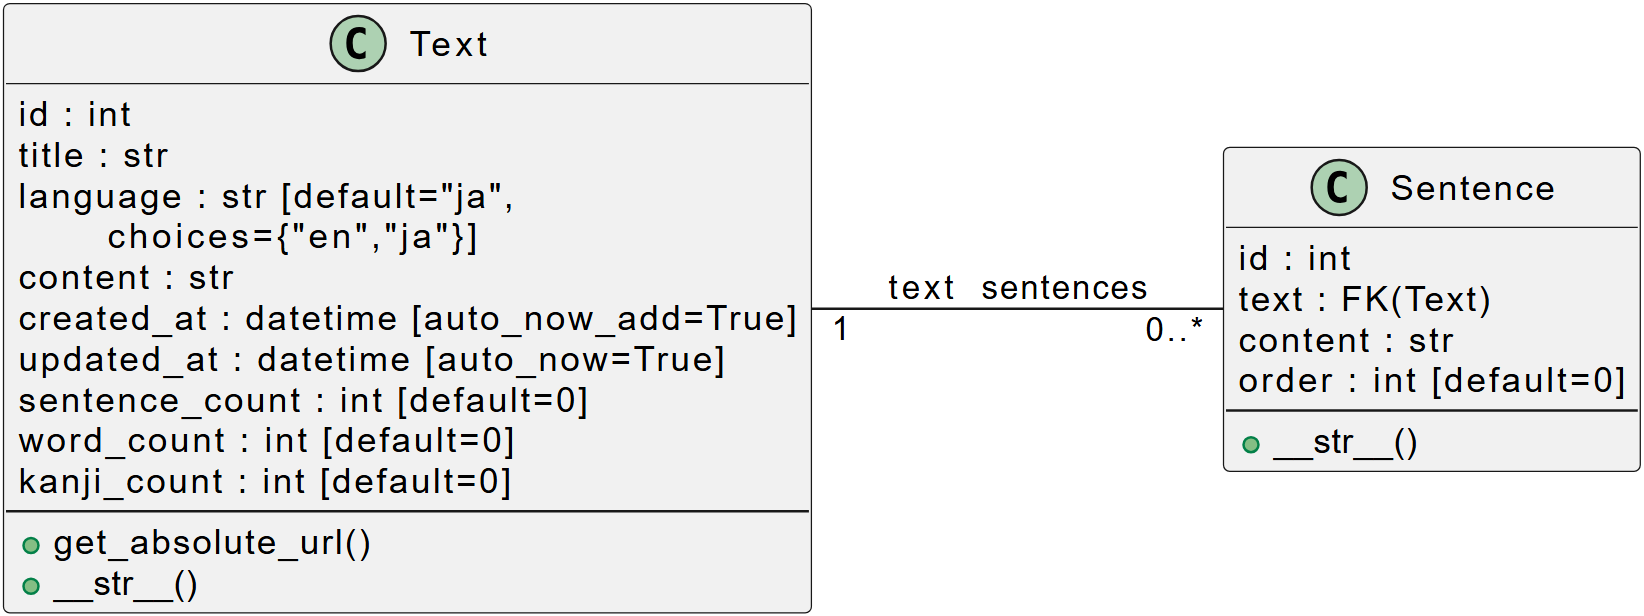
\includegraphics[width=1\textwidth]{images/impl/text_sentence_uml.png}
	\caption{A \texttt{Text} és \texttt{Sentence} osztályok UML modellje}
	\label{fig:text-sentence-uml}
  \end{figure}


  \item \textbf{Word} - Egy mondatban előforduló szó. Az objektum nyelvétől függően, egyes mezők nem kerülnek felhasználásra, egy angol szónak természetesen nincsen kana írásjelű olvasata a \texttt{reading} mezőben.
  \textit{Fő mezők:}
  \begin{itemize}
    \item \texttt{sentences}: Több-mondatos kapcsolat (\textit{ManyToManyField}), vagyis egy szó több mondatban is előfordulhat, és egy mondatban több szó is lehet. Ez a kapcsolat rugalmasabb, mint egy egyszerű \textit{ForeignKey}, és támogatja a szavak újrahasznosítását, keresését.
    \item \texttt{surface\_form}: A szó felszíni alakja, ebben formában jelenik meg a szavak listájában és a szótárakban.
    \item \texttt{lemma\_forms}, \texttt{seen\_forms}: JSON mezők, amelyek a szó lemmáit (alapalakjait) és előforduló alakjait tárolják listákban.
    \item \texttt{pos}, \texttt{meaning}, \texttt{frequency}: Szófaj (\textit{Part of speech}), jelentés és előfordulások száma az eddig elemzett szövegekben.
    \item \texttt{language}: A szó nyelve, csak „en” vagy „ja” lehet, alapértelmezett „ja”.
    \item \texttt{jlpt\_level}, \texttt{cefr\_level}: Nehézségi szint JLPT vagy CEFR szerint.
    \item \texttt{last\_reviewed}, \texttt{next\_review}, \texttt{ease\_factor}, \texttt{interval}, \texttt{repetitions}, \texttt{status}, \texttt{srs\_answer\_history}: A tanulási algoritmus működéséhez szükséges mezők, ezek a következő, Kanji modellben is szerepelnek, ott részletesebben kitérünk rájuk. A teljes UML diagram a \ref{fig:word-uml}.~ábrán szerepel:
  \end{itemize}

  \begin{figure}[H]
	\centering
	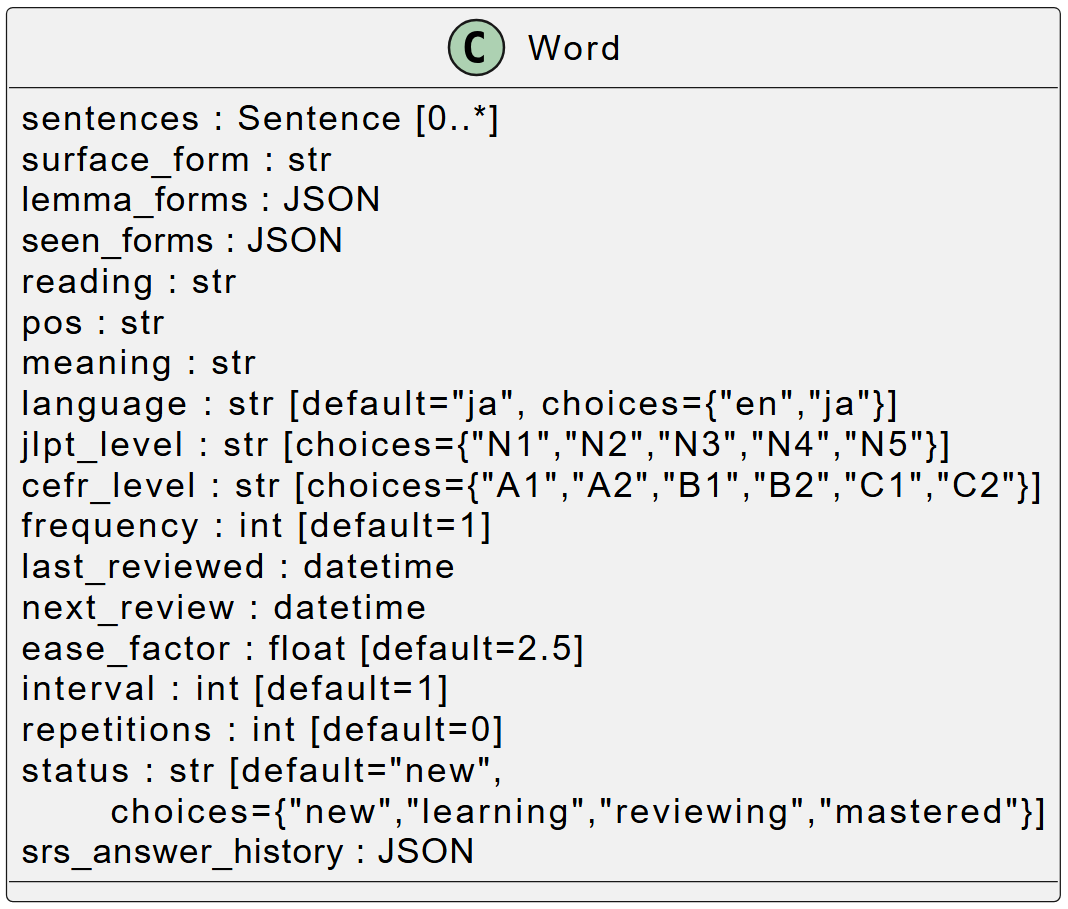
\includegraphics[width=0.675\textwidth]{images/impl/word_uml.png}
	\caption{\texttt{Word} osztály UML modellje}
	\label{fig:word-uml}
  \end{figure}
  
  \item \textbf{Kanji} - Japán karakter. A főbb különbség, a szavak és kanji írásjelek között, hogy egy szövegben egy kanji karakter jelentés nélkül, tulajdonnévként is szerepelhet. Ezért két fő csoportba soroljuk a őket a projektben a \texttt{usage\_type} mező alapján, \textit{name-only}, amelyek személy-, hely-, és egyéb tulajdonnevekben szerepelnek és \textit{productive}, amelyek valódi jelentésüket hordozva jelennek meg. A teljes osztály diagramja a \ref{fig:kanji-uml}.~ábrán látható.
  \textit{Fő mezők:}
  \begin{itemize}
    \item \texttt{words}: Kapcsolódó szavak (ManyToManyField), vagyis egy kanji több szóban is előfordulhat, és egy szóban több kanji is lehet, ez csak a \textit{productive} elemeknél jön létre.
    \item \texttt{texts}: Kapcsolódó szövegek (ManyToManyField), ez csak a \textit{name-only} elemeknél szerepel, hiszen ezek nem tartoznak lexikálisan elemzett szavakhoz.
    \item \texttt{meaning}, \texttt{character}, \texttt{on\_readings}, \texttt{kun\_readings}: A kanji jelentése, maga a karakter, valamint on- és kun-olvasatai (JSON mezők listaként).
    \item \texttt{jlpt\_level}, \texttt{stroke\_count}, \texttt{grade\_level}: Általános statisztikák.
    \item \texttt{general\_frequency}, \texttt{frequency}: Előfordulási gyakoriságok a nyelvben, és a projekten belüli szövegekben
    \item \texttt{last\_reviewed}, \texttt{next\_review}: Az utolsó, és a következő esedékes ismétlések időpontjai
    \item \texttt{ease\_factor}: Tanulási nehézségi szorzó. Alapértelmezetten 2.5 értékű, ez a szám a tanuló válaszai alapján módosul, a következő ismétlés dátumának kiszámításához használjuk.
    \item \texttt{interval}: Az aktuális ismétlés után hány nap múlva esedékes a következő ismétlés.
    \item \texttt{repetitions}:  Az egymást követő sikeres ismétlések száma. Minden helyes válasz után nő, hibás válasz esetén visszaáll 0-ra.
    \item \texttt{status}: Az elem tanulási állapota.
      \begin{enumerate}
          \item \texttt{new}: Új, még nem tanult elem
          \item \texttt{learning}: Éppen tanulás alatt álló elem, amelyre a felhasználó nem adott még helyes választ ami más dátumra helyezné azt.
          \item \texttt{reviewing}: Ismétléses fázisban lévő elem, amely utolsó ismétlés során helyes választ kapott.
          \item \texttt{mastered}: Elsajátított, ritkábban ismétlendő elem amely már nagyon sokszor helyesen lett megválaszolva, így a rendszer ritkán kínálja fel.
      \end{enumerate}
    \item \texttt{srs\_answer\_history}: Az adott elemhez tartozó válaszok (dátum, válaszok listája) naplója.

    \begin{figure}[H]
      \centering
      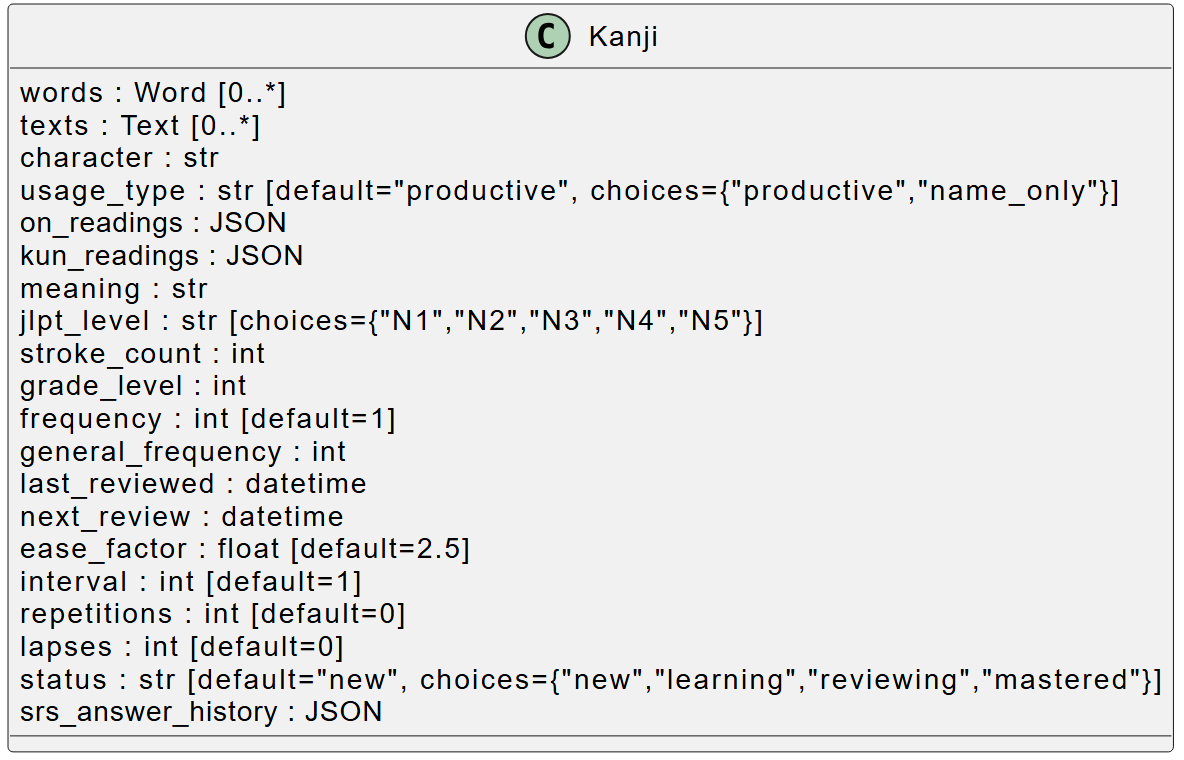
\includegraphics[width=1\textwidth]{images/impl/kanji_uml.png}
      \caption{Kanji osztály teljes diagramja}
      \label{fig:kanji-uml}
\end{figure}
  \end{itemize}


  \item \textbf{Referencia Modellek} - Ezek a modellek kizárólag a hozzájuk tartozó alapmodellek kapcsolódó, külső adatbázisokból vagy szótárfájlokból származó háttéradatokat tárolják, mint az angol szavaknál a nyelvvizsgaszint, japán szavaknál a kanji- és kana-olvasatok, jelentések, JLPT szintek és kanji írásjeleknél a különböző olvasatok, jelentés,  vonásszám, nyelvvizsgaszint, tanult osztály és az Oktatási Minisztérium felmérései által meghatározott előfordulási gyakoriságok.

\end{itemize}

Az alábbi a \ref{fig:er}.~ ábrán megtekinthetők a fő modellek kapcsolatai:

\begin{figure}[H]
  \centering
  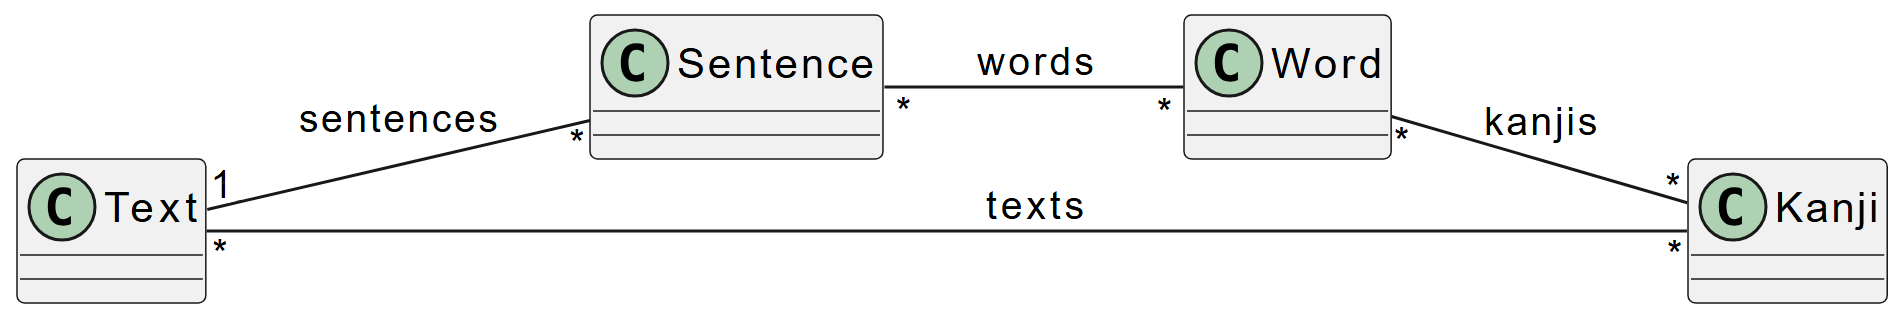
\includegraphics[width=1\textwidth]{images/impl/er.png}
  \caption{Osztályok egyszerűsített kapcsolatai}
  \label{fig:er}
\end{figure}


\paragraph{Management parancsok}

A projektben több olyan háttérfolyamattal rendelkezik, amelyek a referenciaadatok betöltését és frissítését végzik. Ezek a korábban látott Django \textit{management command} formájában lettek megvalósítva, így egyszerűen futtathatók a \texttt{python manage.py <parancs\_neve>} paranccsal. Mindhárom függvény közös jellemzője, hogy nagy mennyiségű külső adatot dolgoz fel (több ezer sort tartalmazó CSV, XML, valamint szótári állományok), ezért az importálás minden esetben bulk módszerekkel történik (\texttt{bulk\_create}, frissítés esetén tömeges update). Ez jelentős teljesítménynövekedést biztosít a Django ORM egyenkénti \texttt{.save()} hívásaival szemben. A projektben megtalálható három parancs és feladatuk a \ref{tab:management} táblázatban látható.

\begin{table}[H]
	\centering
	\begin{tabular}{ | m{0.4\textwidth} | m{0.5\textwidth} | }
		\hline
		\textbf{Parancs} & \textbf{Feladat} \\
		\hline \hline
		\texttt{import\_cefr\_levels} & CEFR szintek beolvasása és az EnglishWordReference tábla feltöltése. \\
		\hline
		\texttt{import\_and\_update\_kanjidic2} &  Kanjidic2 állomány alapján a kanji referenciaadatok importja és frissítése. \\
		\hline
		\texttt{import\_jmdict\_jlpt\_merge} & Japán szótári adatok és JLPT szintek összevonása, WordReference objektumok létrehozása. \\
		\hline
	\end{tabular}
	\caption{Rövid összegzés a management parancsokról}
	\label{tab:management}
\end{table}

\paragraph{Migrációk}

A \texttt{core/migrations} mappa tartalmazza a Django által generált migrációs fájlokat. Ezek automatikus jönnek létre, amikor a modelleken belül változtatások történnek. Ezek feladat a modellek és adatbázis közötti összhang biztosítása, valamint elősegítik a verziók között változtatások átláthatóságát és nyomon követhetőségét. 

\paragraph{Admin nézet}

A \texttt{core/admin.py} felelős a modellekhez tartozó rendszergazdai nézetek regisztrálásáért. A testreszabott admin felület segíti az adatok gyors áttekintését, szerkesztését és karbantartását. Minden fő modellhez külön admin osztály tartozik, amely meghatározza, hogy milyen mezők jelennek meg a listákban, milyen szűrési és keresési lehetőségek vannak, és hogyan jelennek meg az adatok. Például a \texttt{TextAdmin} listázza a szövegek címét, nyelvét, mondat-, szó- és kanji-számát, valamint a létrehozás dátumát.

\subsubsection{A \texttt{dashboard} modul}

A \texttt{dashboard} modul az alkalmazás felhasználói felületének központi vezérlője. Itt történik a szövegek feltöltése, listázása, elemzési folyamatok indítása, valamint a feldolgozott adatok (mondatok, szavak, kanji írásjelek) áttekintése és statisztikák megjelenítése. A \texttt{dashboard} biztosítja a felhasználó számára az elsődleges interakciós pontot, innen indulnak a nyelvi elemzések, és itt lehet böngészni, keresni, illetve részletesen megtekinteni a tanulási és feldolgozási eredményeket. A modul szorosan együttműködik a \texttt{processor} és \texttt{dictionary} appokkal, de a vezérlés és a megjelenítés logikája itt összpontosul.

A \texttt{dashboard} alkalmazás URL-jei és a hozzájuk tartozó nézetek határozzák meg, hogy a felhasználó milyen funkciókat érhet el a rendszerben, és ezek hogyan kerülnek feldolgozásra a backend oldalon. Minden végpont egy adott műveletet vagy oldal megjelenítését szolgálja, amelyhez egy vagy több nézet (függvény vagy osztály) tartozik. Ezek gyakran használnak segédfüggvényeket (\texttt{utils.py} fájl), amelyek a szűrést, exportálást, statisztikák számítását vagy egyéb logikát támogatják.

Az alábbiakban végpontcsoportonként, részletesen bemutatjuk az egyes URL-eket, a hozzájuk tartozó nézeteket, azok fő feladatait, valamint a kapcsolódó segédfüggvényeket és a fontosabb kódrészleteket.

\paragraph{Főoldal (\texttt{/})}

Ez a dashboard kezdőnézete, ahol a felhasználó új szöveget tölthet fel feldolgozásra. A nézet GET kérés esetén a feltöltő űrlapot jeleníti meg, míg POST kéréskor feldolgozza a beadott adatokat. A szöveg forrása lehet közvetlenül beírt tartalom vagy feltöltött fájl, ez utóbbi esetben a rendszer a szövegfeldolgozásért felelős \texttt{processor} modul \texttt{extract\_text\_from\_file()} segédfüggvényét használja a fájl tartalmának kiolvasására.

A nézet a bevitt adatokat validálja, és sikeres feltöltés után létrehoz egy új \texttt{Text} objektumot, majd átirányítja a felhasználót a \texttt{processor} modul feldolgozó nézetéhez. A view AJAX-alapú részleges validációt is támogat (például címmező valós idejű ellenőrzése), amely JSON választ ad vissza. Az alábbi rövid \ref{src:home} kódrészlet bemutatja ennek működését.

\lstset{caption={Főoldal nézet rövid konfigurációja}, label=src:home}
\begin{lstlisting}[language={Python}]
def home(request):
    if request.method == "POST":
        title = request.POST.get("title")
        content = request.POST.get("content")
        uploaded_file = request.FILES.get("upload_file")

        if uploaded_file:
            success, result = extract_text_from_file(uploaded_file)
            if not success:
                messages.error(request, result)
                return render(request, "dashboard/home.html")
            content = result

        if title and content:
            text = Text.objects.create(title=title, content=content)
            return redirect("processor:process_text", text_id=text.id)

    return render(request, "dashboard/home.html")
\end{lstlisting}

\paragraph{Szövegek végpontjai és nézetei}

A Text objektumokkal kapcsolatos végpontok lehetővé teszik a rendszerben tárolt szövegek listázását, részletes megtekintését, törlését, exportálását, illetve összevonását. Az alábbiakban minden végponthoz megadjuk a hozzá tartozó nézetet, rövid leírást, valamint ahol indokolt, egy jellemző kódrészletet.

\begin{itemize}
  \item \textbf{Szövegek listázása (\texttt{/texts/})}
  Ez a végpont jeleníti meg a rendszerben tárolt szövegek listáját, keresési és szűrési lehetőségekkel. A nézet megvalósítása a Django generikus \texttt{ListView} osztályára épül (lásd \ref{src:text-list} ábra).

\lstset{caption={Szövegek listájához tartozó nézet}, label=src:text-list}
\begin{lstlisting}[language={Python}]
class TextListView(ListView):
    model = Text
    template_name = "dashboard/text_list.html"
    context_object_name = "texts"
    ordering = ["-created_at"]
\end{lstlisting}

  \item \textbf{Szöveg részletes nézete (\texttt{/texts/int:pk/})}
  Egy adott szöveg teljes tartalmát jeleníti meg, beleértve a hozzá tartozó szavakat, kanji karaktereket és a statisztikákat. A statisztikai adatok előállítása a \texttt{utils.calculate\_text\_statistics()} segédfüggvénnyel történik. A nézet a listázóhoz hasonlóan a Django \texttt{DetailView} osztályát használja, ezért kódrészlet itt nem szükséges.

  \item \textbf{Szöveg törlése (\texttt{/texts/int:pk/delete/})}
  A törlési folyamat megerősítést kér, majd sikeres végrehajtás után visszairányít a szöveglistára. A megvalósítás a Django \texttt{DeleteView} osztályára épül, külön logika nélkül.

  \item \textbf{Szöveg exportálása (\texttt{/texts/int:text\_id/export/})}
  A kiválasztott szöveghez tartozó adatok exportálása CSV, Excel és Quizlet formátumban. A nézet POST kérés esetén a \texttt{utils.py} exportáló függvényeit hívja meg (pl. \texttt{export\_words\_csv}, \texttt{export\_kanji\_excel}). Sikeres export esetén letölthető fájlt ad vissza, hibás paramétereknél pedig hibaüzenetet jelenít meg. A kód rövid változata a \ref{src:text-export}. számú ködrészletben tekinthető meg:

\lstset{caption={Szöveg exportálás nézet rövid konfigurációja}, label=src:text-export}
\begin{lstlisting}[language={Python}]
def text_export(request, text_id):
    text = get_object_or_404(Text, id=text_id)
    if request.method == "POST":
        export_format = request.POST.get("export_format")
        export_type = request.POST.get("export_type")
        if export_type == "words":
            if export_format == "csv":
                return export_words_csv(words, text.title)
            elif export_format == "excel":
                return export_words_excel(words, text.title)
            # ...
        elif export_type == "kanji":
            if export_format == "csv":
                return export_kanji_csv(kanjis, text.title)
            elif export_format == "excel":
                return export_kanji_excel(kanjis, text.title)
            # ...
    return redirect("dashboard:text_list")
\end{lstlisting}

  \item \textbf{Szövegek összevonása (\texttt{/texts/merge/execute/})} \\
  Ez a végpont teszi lehetővé két szöveg egyesítését. A felhasználó POST kérésben megadja a két szöveg azonosítóját, majd a nézet ellenőrzi, hogy nem ugyanaz-e a két objektum, és azonos nyelvűek-e. Ezt követően a tényleges összevonást a \texttt{merge\_texts()} segédfüggvény végzi. Sikeres művelet után az új szöveg automatikusan feldolgozásra kerül. Ennek a folyamatnak rövidített verziója a \ref{src:text-merge}. számú forráskódban látható.

\lstset{caption={Szövegek összevonása nézet rövid konfigurációja}, label=src:text-merge}
\begin{lstlisting}[language={Python}]
def text_merge_execute(request):
    if request.method == "POST":
        text1_id = request.POST.get("text1_id")
        text2_id = request.POST.get("text2_id")
        if not text1_id or not text2_id or text1_id == text2_id:
            return redirect("dashboard:text_list")
        text1 = get_object_or_404(Text, id=text1_id)
        text2 = get_object_or_404(Text, id=text2_id)
        if text1.language != text2.language:
            return redirect("dashboard:text_list")
        merged_text = merge_texts(text1, text2)
        return redirect("processor:process_text", text_id=merged_text.id)
    return redirect("dashboard:text_list")
\end{lstlisting}

\end{itemize}

\paragraph{Szavak végpontjai és nézetei}

\begin{itemize}
  \item \textbf{Szavak listázása (\texttt{/words/})}
  Ez a végpont jeleníti meg a rendszerben tárolt szavak listáját, keresési, szűrési, valamint szótárakhoz való hozzárendelési lehetőségekkel. A nézet a Django generikus \texttt{ListView} osztályára épül, kiegészítve egyedi query logikával. Ennek működését az alábbi \ref{src:word-list}. számú kódrészletben szereplő \texttt{due\_today} GET paraméteren keresztül fogjuk szemléltetni. Ez jelzi azt, hogy csak azon szavakat szeretnénk látni a listában, amelyek \texttt{next\_review} paramétere a mai napra esik. A \ref{src:due-today}. részen látható \texttt{apply\_due\_today\_filter} util valósítja meg ezt a logikát, ha a \texttt{due\_today} be van állítva, akkor a querysetben csak a kívánt elemek maradnak. 
    
\lstset{caption={Szavak listájához tartozó nézet}, label=src:word-list}
\begin{lstlisting}[language={Python}]
class WordListView(ListView):
    model = Word
    template_name = "dashboard/word_list.html"
    context_object_name = "words"
    ordering = ["-id"]
    paginate_by = 30
    def get_queryset(self):
        current_language = self.request.GET.get("language", "ja")
        queryset = Word.objects.filter(language=current_language)
        # ... query logika ...
        due_today = self.request.GET.get("due_today")
        queryset = apply_due_today_filter(queryset, due_today, "next_review")
        # ... query logika ...
        return queryset
\end{lstlisting}

\lstset{caption={Mai napra szűréskor használt segédfüggvény}, label=src:due-today}
\begin{lstlisting}[language={Python}]
def apply_due_today_filter(queryset, due_today, field_name):
    if due_today:
        today = timezone.now().date()
        return queryset.filter(**{f"{field_name}__date": today})
    return queryset
\end{lstlisting}

  \item \textbf{Szó részletei (\texttt{/words/int:word\_id/})}
  Ez a végpont egy adott szó részletes adatlapját jeleníti meg, beleértve a hozzá tartozó statisztikákat és a szótárakhoz való hozzárendelés lehetőségét. A nézet a Django generikus \texttt{DetailView} osztályára épül, így külön kód részletet nem igényel.

  \item \textbf{Szó hozzáadása szótárakhoz (\texttt{/words/add-to-dictionaries/})}\label{word-add}
  Ez a végpont lehetővé teszi, hogy egy kiválasztott szót egy vagy több szótárhoz rendeljünk hozzá. Egy POST kérést vár, amely tartalmazza a szó azonosítóját és a kiválasztott szótárak listáját. A  módon a nézet ellenőrzi, hogy a kérésben szerepel-e mind a szó, mind a szótár vagy szótárak azonosítója, majd elvégzi a hozzárendelést. 

  \item \textbf{Tömeges szóhozzáadás szótárakhoz (\texttt{/words/bulk-add-to-dictionaries/})}\label{word-add-bulk}
  Egy szűrési feltételeknek megfelelő összes szót egyszerre több szótárhoz rendeljük. A szinguláris szó hozzáadásához hasonlóan a kiválasztott szótárak listáját és opcionálisan a további szűrési beállításokat várja paraméterül.

\end{itemize}

\paragraph{Kanji karakterek végpontjai és nézetei}

A Kanji objektumokhoz kapcsolódó végpontok felépítése és működése nagyban hasonlít a \texttt{Word} modell esetében bemutatottakhoz. A két struktúra azonos logikát követ, szerepel benne listázás, részletek megjelenítése, valamint egyedi és tömeges szótárhoz rendelés. A különbség kizárólag az adatszerkezetben rejlik, ugyanis itt több lexikális adattal dolgozik a rendszer (olvasatok, összetevők, vonásszám), de a végpontok kezelési módja változatlan.

\begin{itemize}
  \item \textbf{Kanji karakterek listázása (\texttt{/kanji/})}
  A Word osztály listázásával megegyezően működő végpont, kiegészítve a karakterekre jellemző szűrési és rendezési paraméterekkel.

  \item \textbf{Kanji részletei (\texttt{/kanji/int:kanji\_id/})}
  Szavak részletes nézeteivel megegyező alapon működik, egy adott írásjelhez tartozó adatok, statisztikák és szótárba rendezési lehetőségek jelennek meg.

  \item \textbf{Kanji hozzáadása szótárakhoz (\texttt{/kanji/add-to-dictionaries/})}
  A működése megegyezik a szavaknál alkalmazott szótár hozzárendeléssel. POST kérésben kapott azonosítókat dolgoz fel, és létrehozza a kapcsolódó bejegyzéseket.

  \item \textbf{Tömeges hozzáadás szótárakhoz (\texttt{/kanji/bulk-add-to-dictionaries/})}
  A szóalapú tömeges művelet analógja. A megadott szűrési feltételeknek megfelelő összes kanji egyszerre kerül hozzárendelésre a kijelölt szótárakhoz.
\end{itemize}
  
\paragraph{\texttt{dashboard/templatetags}}

A \texttt{dashboard/templatetags/dashboard\_filters.py} egyedi Django template filtereket és tageket tartalmaz, amelyek a dashboard HTML sablonjaiban segítik az adatok formázását és a dinamikus URL-kezelést. Ezek a segédfüggvények javítják a felhasználói élményt és átláthatóbbá teszik a felületet. Többek között a NLP csomagok által a szavakhoz csatolt szófajokat (például \begin{CJK}{UTF8}{min}名詞, 動詞\end{CJK}, NOUN, VERB) angol nyelvű, felhasználóbarát elnevezéssé, a felhasználó által ismétlések során adott válaszkódokat (0–3) szöveges értékké alakítja (\textit{Again}, \textit{Hard}, "\textit{Good}, \textit{Easy}). Ezen kívül az itt lévő rövid függvények segítségével a sablonokban dinamikusan lehet URL paramétereket hozzáadni, módosítani vagy eltávolítani, például szűrők és rendezések kezeléséhez.

\subsubsection{A \texttt{processor} modul}

A \texttt{processor} modul a LanDB alkalmazás legfontosabb háttérkomponense, amely a nyers szövegek automatikus feldolgozását, nyelvi elemzését és az adatbázisba történő strukturált betöltését végzi. Ez a modul hidat képez a felhasználói adatbevitel (szövegfeltöltés vagy beírás) és a tanulási, adminisztrációs funkciók között, biztosítva, hogy a rendszerben minden nyelvi adat egységes, kereshető és statisztikailag feldolgozható formában jelenjen meg.

\paragraph{Általános feldolgozási folyamat}

A szövegfeldolgozás folyamata a következő logikai lépésekből áll:

\begin{enumerate}
    \item A bemenet validálása, figyelembe véve az üres tartalmat, karakterkészletet és fájltípust.
    \item A szöveg előfeldolgozása, ideértve a fájlból való kiolvasást a megfelelő formátumokból.
    \item A nyelv azonosítása és szöveg mondatokra tagolása.
    \item Tokenizálás, a nyelvnek megfelelő eszközök alkalmazásával.
    \item A szófaj és más nyelvi jellemzők meghatározása.
    \item Egyedi szó és kanji objektumok létrehozása vagy frissítése.
    \item Mondat–szó, valamint szó–kanji kapcsolatok tárolása.
    \item A statisztikák frissítése.
\end{enumerate}

A teljes folyamat során tömbösített, optimalizált mentési műveleteket használunk (\texttt{bulk\_create}, \texttt{bulk\_update}), amelyek jelentősen csökkentik az adatbázis műveletek költségét.

\paragraph{URL-végpontok}

\begin{itemize}
    \item \texttt{/validate-content/}: AJAX-alapú tartalom ellenőrzés (üres-e, felismerhető-e a nyelv).
    \item \texttt{/process/<id>/}: a teljes szövegfeldolgozási folyamat indítása.
\end{itemize}

Ezek a végpontok kizárólag a vezérlő szerepét töltik be, a tényleges
nyelvi feldolgozás a \texttt{utils.py}-ban található segédfüggvényeken keresztül történik.

\paragraph{A feldolgozást végző nézetek}

A folyamat központi eleme a \texttt{process\_text} nézet, amely meghatározza, hogy a szöveget japán vagy angol feldolgozó futtatja tovább. 

\begin{itemize}
    \item \textbf{\texttt{process\_japanese\_text()}}: MeCab-alapú
    tokenizálás, lemma és szófaji címkék meghatározása, kanji kigyűjtése,
    Word–Kanji kapcsolatok létrehozása. Ez a kód a \ref{src:process-japanese-text} számú kódrészletben látható.
    \item \textbf{\texttt{process\_english\_text()}}: spaCy-alapú
    tokenizálás, lemma és szófaj meghatározása, automatikus magyar fordítás
    (\texttt{Deep Translate és googletrans}), CEFR-szintek hozzárendelése.
\end{itemize}

Mindkét függvény azonos lépéseket hajt végre, de különböző eszközökkel. Elsőként a mondatokat hozza létre, majd mentésük után szavak összegyűjtése és normalizálása következik. Ezt követően az új szavakat felvesszük az adatbázisba, a már meglévőeket frissítjük a mondat-szó kapcsolatok rögzítésével. Ezután frissítjük a statisztikákat, mint mondatok és szavak számai és előfordulásaik. A feldolgozás legnagyobb része a \texttt{utils.py}-ban található segédfüggvényeken keresztül történik. Ezek külön funkcionális kategóriákra bonthatók:

\begin{itemize}
    \item \textbf{Fájlkezelés}: \texttt{extract\_text\_from\_file()} támogatja
    a .txt, .pdf, .docx formátumok beolvasását, hibakezeléssel.
    
    \item \textbf{Validáció}: \texttt{is\_japanese()}, \texttt{is\_english()}, \texttt{validate\_content()} ellenőrzik a bemenet érvényességét egyszerű reguláris kifejezesék segítségével. Ezek a \ref{src:regex} kódrészletben láthatók:

\lstset{caption={Regex ellenőrzések szövegek nyelvi tartalmához}, label=src:regex}
\begin{lstlisting}[language={Python}]
def is_english(text):
    return re.search(r"[a-zA-Z]", text) is not None

...

def is_japanese(text):
    return re.search(r"[\u3040-\u30FF\u4E00-\u9FFF]", text) is not None
\end{lstlisting}
    
    \item \textbf{Mondatfelosztás és tokenizálás}: \texttt{split\_japanese\_sentences()} és \texttt{split\_english\_sentences()} nyelvspecifikus szabályokat alkalmaznak a mondatvégi karakterek eltérése miatt. Majd japán esetén MeCab, angol esetén spaCy alapú feldolgozás következik, amely tartalmazza a lemma, szófaj és olvasat meghatározását. Itt főleg a japán karakterekre fontosabb szűréseket kell tenni, ezt végzik többek között a \texttt{is\_named\_entity(pos1)} (tulajdonnevek felismerése), \texttt{is\_te\_iru\_or\_aru(lemma, prev)} (segédigék kiszűrése), \texttt{extract\_surface\_form()} (felszíni alak kivonása) függvények is.

    
    \item \textbf{Adatbázis műveletek}:  
    A feldolgozott szavak és mondatok adatbázisba mentését több, kimondottan erre tervezett függvény végzi. Ezek egymás utáni működése a \texttt{process\_japanese\_text(request, text)}-t leíró, \ref{src:process-japanese-text} számú kódrészletben jól látható. A \texttt{save\_japanese\_sentences()} létrehozza az adott szöveghez tartozó mondatobjektumokat, a \texttt{save\_japanese\_words()} eltárolja az alapszó adatait és azok előfordulási gyakoriságát, míg a \texttt{save\_kanjis()} a produktív és névelemként előforduló írásjeleket rögzíti a \texttt{Kanji} táblában. Az ezt követő lépésben a \texttt{link\_japanese\_words\_to\_sentences()} a megfelelő mondatokhoz rendeli a szavakat, majd hozzájuk a \texttt{link\_kanjis\_to\_words()} csatolja az írásjeleket. A csak névelemként előforduló karakterek közvetlenül a szöveghez kapcsolódnak (\texttt{link\_name\_only\_kanjis\_to\_text()}). A feldolgozás végén az \texttt{update\_japanese\_text\_statistics()} frissíti a főbb statisztikákat, majd a felhasználó átirányításra kerül a \texttt{TextView} nézetre.

\lstset{caption={Japán szövegek feldolgozása}, label=src:process-japanese-text}
\begin{lstlisting}[language={Python}]
def process_japanese_text(request, text):
    result = tokenize_japanese_text(text.content)

    all_kanji_chars = (
        result["kanji_usage"]["productive"] + result["kanji_usage"]["name_only"]
    )
    word_frequencies, kanji_frequencies = calculate_japanese_frequencies(
        result["sentences"], result["lemmas"], all_kanji_chars
    )

    sentences = save_japanese_sentences(text, result["sentences"])
    words = save_japanese_words(result["lemmas"], word_frequencies)
    kanjis_by_char = save_kanjis(result["kanji_usage"], kanji_frequencies)

    word_connections = link_japanese_words_to_sentences(words, sentences)
    kanji_connections = link_kanjis_to_words(words, kanjis_by_char)

    link_name_only_kanjis_to_text(
        text, kanjis_by_char, result["kanji_usage"]["name_only"]
    )

    stats = update_japanese_text_statistics(text)

    return redirect("dashboard:text_view", pk=text.id)
\end{lstlisting}

\end{itemize}

A \texttt{processor} modul így biztosítja, hogy a nyers szövegből strukturált, kereshető és tanulható adatbázis épüljön fel, támogatva mind a japán, mind az angol nyelvű tanulási folyamatokat.

\subsubsection{A \texttt{dictionary} modul}

Ez a modul az alkalmazás szótárkezelő rendszere, amely lehetővé teszi a tanulókártya-gyűjtemények létrehozását, kezelését, tanulását és exportálását.

\paragraph{Modellek}

A \texttt{models.py} fájl tartalmazza a szótárak adatbázis-modelljeit:

\begin{itemize}
  \item \textbf{Dictionary} - Egy szótár, amely szavakból vagy kanji karakterekből álló tanulókártya-gyűjtemény. Fontos megjegyezni, hogy egy szótár nem tárol vegyes tartalmat, egyszerre csak azonos nyelvű szavak vagy írásjelek lehetnek benne. Ez az egyszerűsítés megkönnyíti mind a felhasználói felület, mind a backend-oldali export- és tanulási logikák kezelését.
  \textit{Fő mezők}:
  \begin{itemize}
    \item \texttt{name}, \texttt{description}: A szótár létrehozáskor kötelezően megadott neve és opcionális leírása.
    \item \texttt{language}: A szótár nyelve, alapértelmezetten japán.
    \item \texttt{content\_type}: A szótárban tárolt nyelvi elem típusa
    \item \texttt{daily\_new\_items}: Napi új tanulókártyák limitje
    \item \texttt{max\_reviews\_per\_day}: Napi ismétlések maximális száma
    \item \texttt{words}, \texttt{kanjis}: Két Many–to–many mezőt tartalmaz
  \end{itemize}

  \item \textbf{DailyStudyStats} - Ez az osztály rögzíti a szótárankénti napi tanulási aktivitást és előzményeket.
  \textit{Fő mezők}:
  \begin{itemize}
    \item \texttt{dictionary}: Hivatkozás a hozzá tartozó szótárra.
    \item \texttt{date}: A tanulási folyamat napja dátuma.
    \item \texttt{new\_items\_studied}: Az adott napon elsajátított új elemek száma.
    \item \texttt{reviews\_done}: Az elvégzett ismétlések száma.
  \end{itemize}
  A modellben szereplő \texttt{unique\_together = (dictionary, date)} megkötés kikényszeríti, hogy minden szótárhoz egy nap csak egy statisztikai bejegyzés tartozhasson, a tanulási folyamat konzisztenciája érdekében. 

\end{itemize}

\paragraph{Végpontok a \texttt{dictionary} modulban}

Ezen végpontok teszik lehetővé a szótárak teljes körű kezelését, tanulását, exportálását és statisztikák lekérdezését. Az URL-ek és a hozzájuk tartozó nézetek a következő fő funkciókat fedik le:

\begin{itemize}
  \item \textbf{Szótárak listázása (\texttt{/dictionaries/})} A felhasználó összes szótárának listázása, statisztikákkal. A nézet a Django generikus \texttt{ListView} osztályára épül.
  \item \textbf{Szótár részletei (\texttt{/dictionaries/<id>/})} Az alapértelmezett DetailView nézetre épül, itt van lehetőség adott szótár tartalmának megtekintésére tanlási statisztikákkal. Itt van lehetőség az elemek eltávolítására a szótárból, valamint a leírás és napi tanulandó ismeretlen szavak korlátjának beállítására.
  \item \textbf{Szótár létrehozása üresen és szövegből (\texttt{/dictionaries/create/empty/} és \texttt{/dictionaries/create/from-text/<text\_id>/})}  Új szótár készítése manuálisan vagy egy Text összes kiválasztott paraméterű objektuma alapján.
  \item \textbf{Szótár törlése} (\texttt{/dictionaries/<id>/delete/}) Az objektum és hozzá tartozó tanulási statisztikák törlése a Django által biztosított DeleteView segítségével.
  \item \textbf{Szótárak egyesítése} (\texttt{/dictionaries/merge/execute}) Szövegekhez hasonló módon a POST kérés alapján megadott két szótár egyesítése, hogyha a paramétereket ellenőrző validálás sikeres volt.
  \item \textbf{Szótár exportálása} (\texttt{/dictionaries/<id>/export/}) Szótár tartalmának exportja CSV, Excel vagy Quizlet formátumban, a szövegeknél látott logika alapján.
  \item \textbf{Elem eltávolítása szótárból} (\texttt{/dictionaries/<id>/remove-item/})  Egy adott szó vagy kanji törlése a szótárból, a kiválasztott elem a POST kérésben kerül átadásra.
  
\end{itemize}

\paragraph{Tanulási logika és algoritmus}

A tanulási funkciók a \texttt{dictionary} alkalmazás leglényegesebb elemei. A rendszer az Anki által inspirált SRS algoritmust használja, amelyet a backendben több, egymással együttműködő függvény valósít meg. A modul négy, kifejezetten tanulásra használt végpontot tartalmaz:

\begin{itemize}
  \item \textbf{Tanulási nézet (\texttt{/dictionaries/<id>/study})} A tanulási nézetet megjelenítő fő oldal, itt igazi algoritmusok és folyamatok nem hajtódnak végre. A szükséges adatokat AJAX-hívásokkal tölti be, így a tanulás folyamatos és oldalfrissítés nélküli. Főként egy UI keretet biztosít a többi funkció megjelenítéséhez. 
  \item \textbf{Tanulási adatok lekérése (\texttt{/dictionaries/<id>/study-data})} Ez a végpont adja vissza az adott tanulási körben használandó kártyákat. A logika a \texttt{utils.py get\_items\_for\_study(dictionary)} segédfüggvényére épül, itt kerül meghatározásra, hogy a tanuló milyen sorrendben kapja meg a kártyákat. Először az esedékes reviewing elemek, majd az új elemek (napi korlát alapján), végül a közel esedékes learning kártyák kerülnek sorra. A felület mindig előre megjeleníti, hogy egy adott kártyánál milyen következő időpontok várhatók, ezt a \ref{src:intervals}. számú kódrészletben látott segédfüggvénnyel tesszük.

\lstset{caption={Következő intervallumok meghatározása}, label=src:intervals}
\begin{lstlisting}[language=Python]
def calculate_next_intervals(item):
    was_new = item.status == "new"
    was_learning = item.status == "learning"
    intervals = {}

    if was_new:
        intervals = {0: "1m", 1: "5m", 2: "10m", 3: "2d"}
    elif was_learning:
        intervals = {0: "1m", 1: "5m", 2: "1d", 3: "4d"}
    else:
        hard = max(1, int(item.interval * 1.2))
        good = max(1, int(item.interval * item.ease_factor))
        easy = max(1, int(item.interval * item.ease_factor * 1.3))

        intervals = {
            0: "1m",
            1: format_interval(hard),
            2: format_interval(good),
            3: format_interval(easy)
        }

    return intervals
\end{lstlisting}

  \item \textbf{Válaszok feldolgozása (\texttt{/dictionaries/<id>/answer})} Az \texttt{update\_item\_after\_answer()} metódus valósítja meg a teljes Anki-szerű SRS logikát. Frissíti az \texttt{ease\_factor} paramétert, az intervallumot, kezeli a státuszok közötti átmeneteket (new $\rightarrow$ learning $\rightarrow$ reviewing), valamint a napi tanulási statisztikákat. Az algoritmus terjedelme miatt az alábbi \ref{src:update-item} kódrészletben csak a fő szerkezeti blokkokat mutatjuk be:

\lstset{caption={SRS frissítés válasz után (rövidített)}, label=src:update-item}
\begin{lstlisting}[language=Python]
def update_item_after_answer(item, difficulty, dictionary):
    now = timezone.now()
    today = date.today()
    was_new = item.status == "new"
    was_learning = item.status == "learning"

    if dictionary:
        daily_stats = get_or_create_daily_stats(dictionary, today)
        
    item.last_reviewed = now

    if difficulty == 0:  # Again -> restart
        item.status = "learning"
        item.repetitions = 0
        item.ease_factor = max(1.3, item.ease_factor - 0.2)

        if was_new and dictionary:
            daily_stats.new_items_studied += 1
            daily_stats.save()

        item.interval = 1 / 1440  # 1 perc
        item.next_review = now + timedelta(minutes=1)
        ...
    else:
        # Hard / Good / Easy esetek
        ...
        
    if item.interval >= 21 and item.status == "reviewing":
        item.status = "mastered"

    item.save()
\end{lstlisting}

  \item \textbf{Napi statisztikák (\texttt{/dictionaries/<id>/study-stats})} Az itt használt \texttt{get\_study\_stats()} függvény összegyűjti a tanulási felülethez szükséges napi statisztikákat mint az új kártyák száma, tanulási státuszok arányai, és esedékes review-k száma..

\end{itemize}

\subsubsection{Sablonok és statikus fájlok}

Az alkalmazás sablonjai (\texttt{templates/}) és statikus fájljai (\texttt{static/}) modulonként felosztott mappastruktúrában helyezkednek el. A teljes felület a\texttt{ base.html} sablonra épül, amely meghatározza az alkalmazás egységes megjelenését, betölti a szükséges CSS/JS könyvtárakat (TailwindCSS, DaisyUI, DataTables), valamint tartalmazza a globális navigációs sávot és a fő tartalmi blokkokat. Minden egyes oldal ebből a sablonból öröklődik, és csak a \texttt{content} és \texttt{scripts} blokkokat tölti fel az adott funkciónak megfelelő HTML-lel és JavaScript-el. Ezt a felépítést \ref{src:word-list.html}. számú kódrészlet jól szemlélteti. Az alkalmazás oldalai közötti navigációt a \ref{fig:navigation}. számú ábra mutatja be. 



\begin{figure}[H]
  \centering
  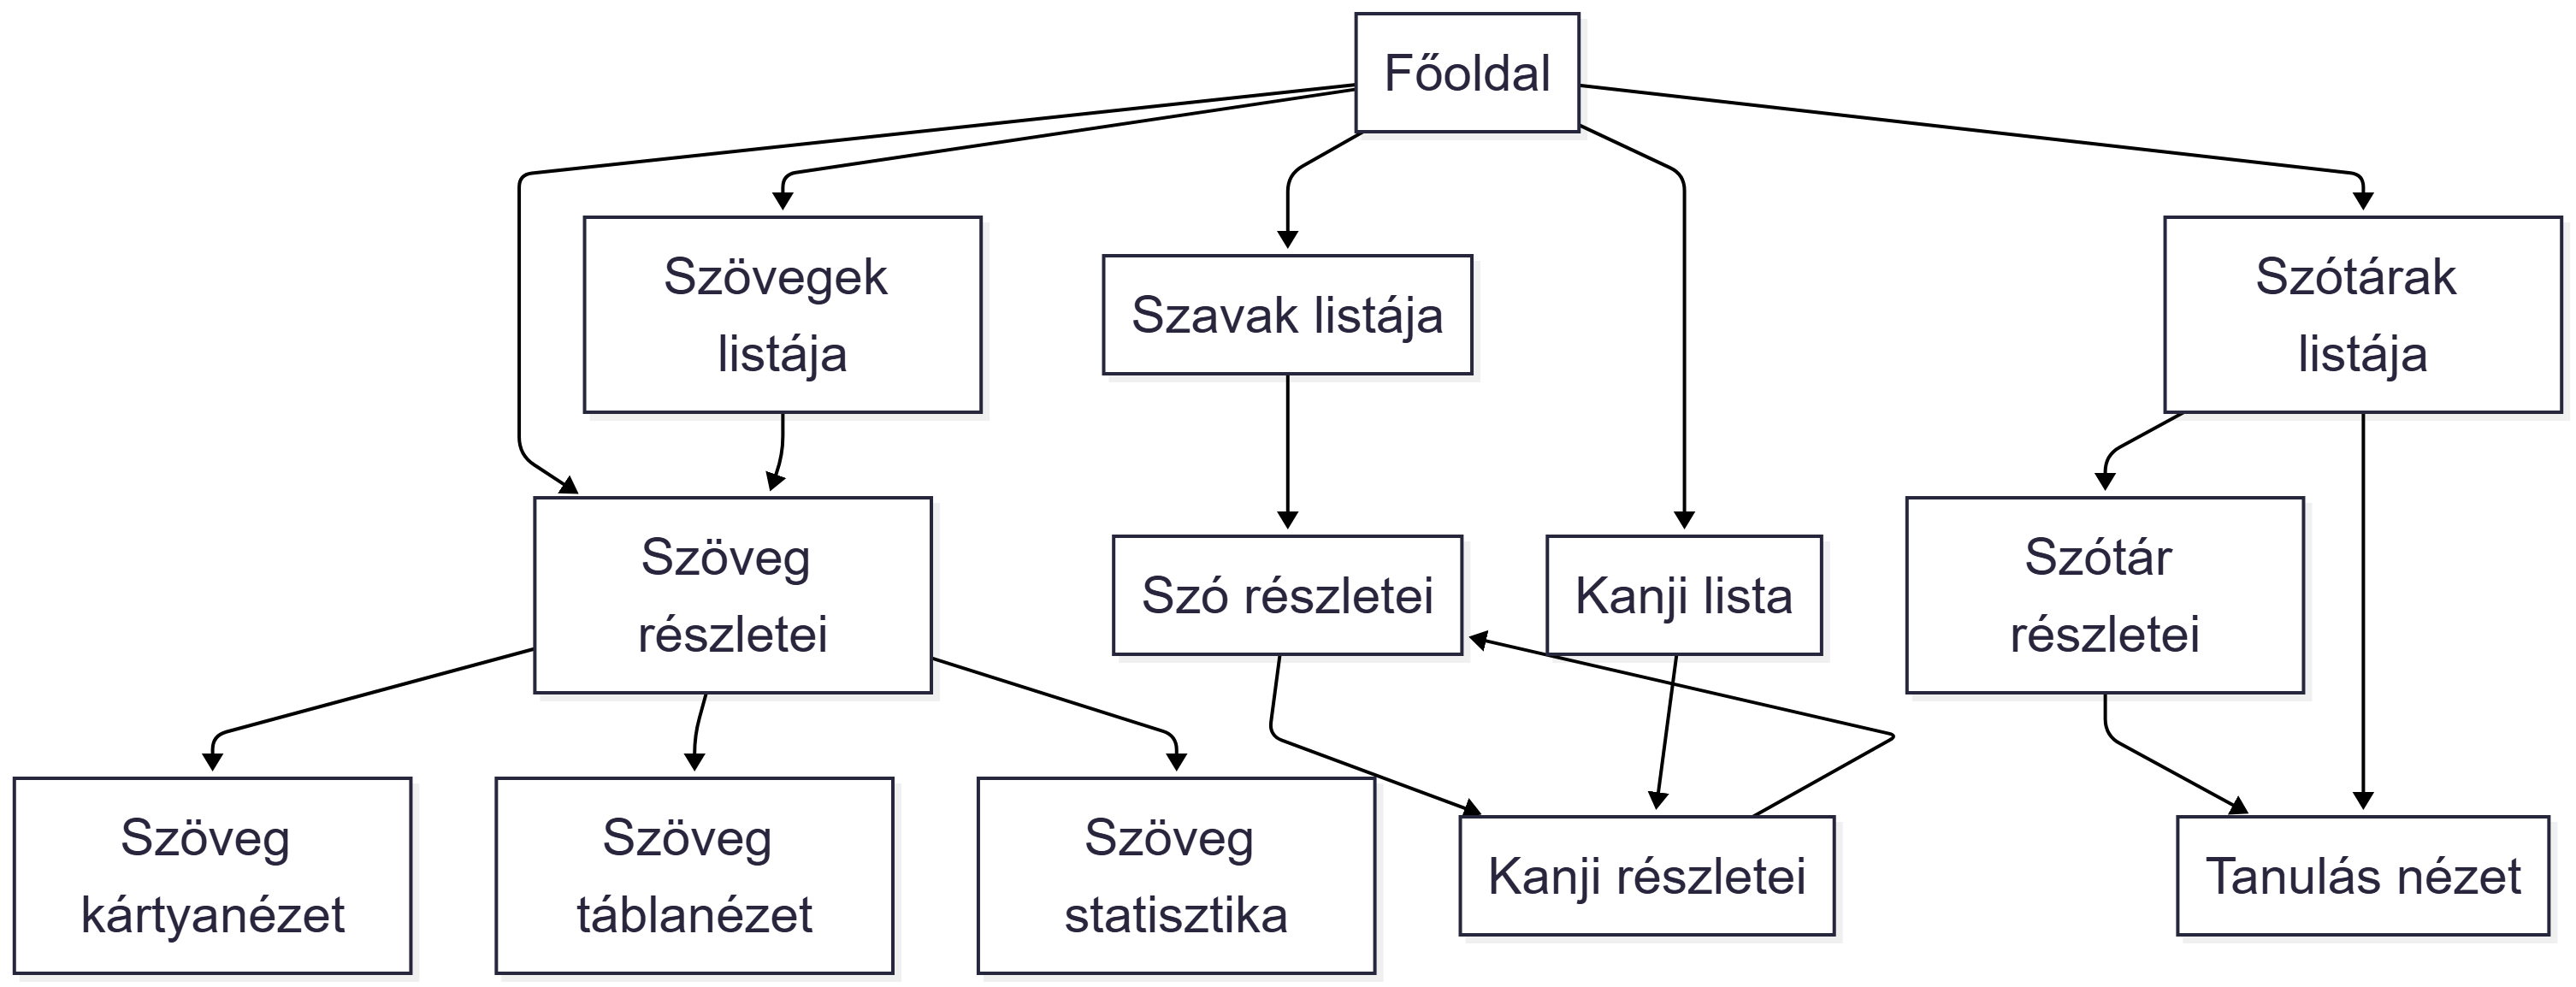
\includegraphics[width=1\textwidth]{images/impl/navigation_map.png}
  \caption{Oldalak navigációs térképe}
  \label{fig:navigation}
\end{figure}

\paragraph{Főoldal}

Ezen a sablonon keresztül a felhasználó új szöveget vihet fel feldolgozásra. Az oldal központi eleme egy űrlap, amelyben megadható a szöveg címe, nyelve (japán vagy angol) valamint maga a szöveg (beillesztve vagy feltöltött fájlból). A sablon a \texttt{base.html}-ből öröklődik, így tartalmazza a globális navigációt, stílusokat és a szükséges blokkokat.

A hozzá tartozó JavaScript (\texttt{home.js}) gondoskodik az űrlap mezőinek valós idejű validálásáról, amely hibák esetén az oldal végén behúzott dialógus sablonon (\_validation\_dialog.html) keresztül figyelmezteti a felhasználót.

\paragraph{Szövegek fő oldalai:}

\begin{itemize}
  \item \textbf{Szövegek listája (\texttt{text\_list.html})}
  Ez a fájl kezeli a szövegek listázó oldalán az exportálást, szótárakká alakítást, egyesítést és törlést. Egyesítésnél a hozzá tartozó \texttt{text\_list.js} szkript segítségével csak az azonos nyelvű szövegeket van lehetőség kijelölni, így bár a backend hibás POST kérés esetén rendelkezik ellenőrzéssel, a felhasználó ezt nem tudja közvetlenül kikényszeríteni. Az összes funkció működését megerősítést igénylő dialógusok segítik, ezek az \texttt{includes} mappában találhatók.

  \item \textbf{Szöveg részletei (\texttt{text\_view.html})}
  Itt kerülnek az adott szöveghez tartozó mondatok, szavak, kanji karakterek és statisztikák megjelenítésre. Többféle megjelenítési mód (kártyanézet, statisztika, táblázat) között lehet váltogatni, ahonnan az egyes elemekre tovább lehet navigálni. A három oldal közötti váltást a \texttt{view\_switcher} komponens segíti elő. Ezek kapcsolatai a \ref{fig:text-nav} ábrán láthatók.

\end{itemize}

\begin{figure}[H]
  \centering
  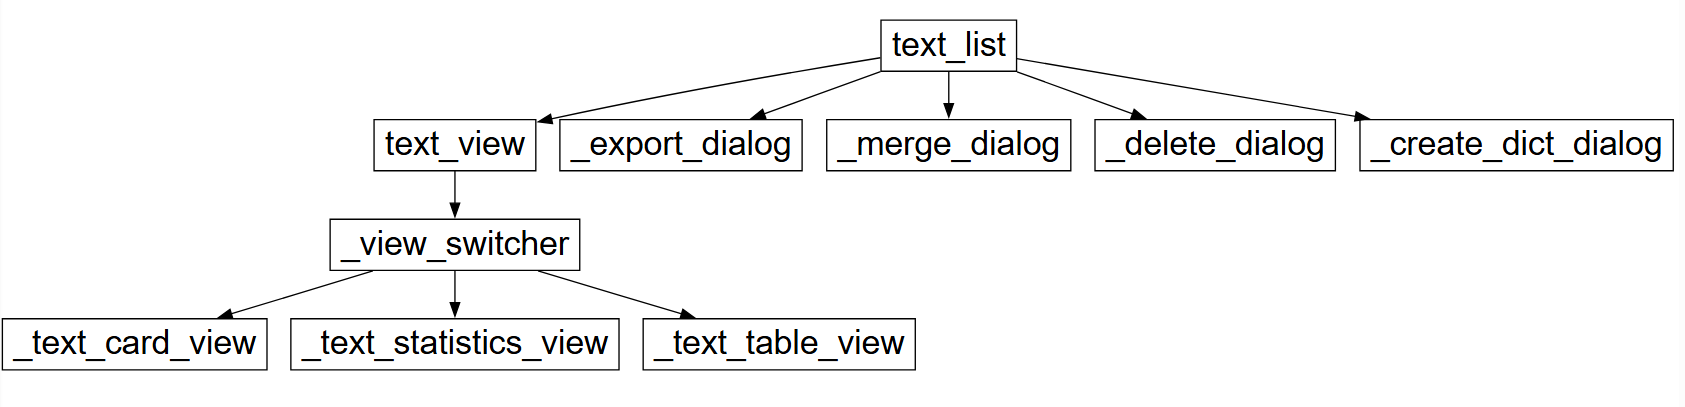
\includegraphics[width=1\textwidth]{images/impl/text_htmls.png}
  \caption{Szövegekhez tartozó HTML sablonok kapcsolatai}
  \label{fig:text-nav}
\end{figure}

\paragraph{Szó és kanji elemek fő oldalai:}

\begin{itemize}
  \item \textbf{Szavak és kanji karakterek listája (\texttt{word\_list.html, kanji\_list.html})}
  Ezek az oldalak jelenítik meg az összes szót (nyelv szerint szétválasztva, a \ref{src:word-list.html}. kódrészletben látott módon) és az összes kanji karaktert, fejlett szűrési, keresési és rendezési lehetőségekkel. A felhasználó szűrhet többek között nyelvvizsgaszint, szófaj, státusz, gyakoriság, szöveg, és dátum szerint, valamint lapozhat a találatok között. Minden elem mellett található egy gomb, amellyel a szó vagy kanji hozzáadható egy szótárhoz (modális dialógusban), illetve lehetőség van az összes szűrt elem tömeges hozzáadására is. Ezekhez az \texttt{includes} mappában található dialógusok tartoznak (\_add\_word\_dialog.html, \_bulk\_add\_word\_dialog.html, \_add\_kanji\_dialog.html, \_bulk\_add\_kanji\_dialog.html). Az oldalak működését a \texttt{list\_common.js} segíti, amely a dialógusok megnyitását, bezárását és a lista rendezésért felelős gombon lévő nyíl irányának cseréjét ($\uparrow$ / $\downarrow$) végzi. A listaoldalakról egy kattintással elérhető az adott szó vagy kanji részletes nézete, ahol további kapcsolódó elemekhez lehet navigálni (szó $\rightarrow$ kanji, kanji $\rightarrow$ szó).

\lstset{caption={A \texttt{word\_list.html} sablon kódja}, label=src:word-list.html}
\begin{lstlisting}[language=html]
{% extends 'base.html' %}
{% load static %}
{% load dashboard_filters %}

{% block title %}Words{% endblock %}

{% block content %}

<div class="flex justify-center mb-4">
    <div class="join">
        <a href="?language=ja" class="join-item btn {% if current_language == 'ja' %}btn-active{% endif %}">
            Japanese ({{ jp_count }})
        </a>
        <a href="?language=en" class="join-item btn {% if current_language == 'en' %}btn-active{% endif %}">
            English ({{ en_count }})
        </a>
    </div>
</div>

{% if current_language == 'ja' %}
    {% include "dashboard/includes/_jp_words_list.html" %}
{% elif current_language == 'en' %}
    {% include "dashboard/includes/_en_words_list.html" %}
{% endif %}

{% endblock %}

{% block scripts %}
<script src="https://unpkg.com/lucide@latest"></script>
<script>lucide.createIcons();</script>
<script src="{% static 'js/dashboard/list_common.js' %}"></script>
{% endblock %}
\end{lstlisting}

  \item \textbf{Szavak és kanji karakterek oldalai (\texttt{text\_list.html, word\_list.html}) }
  Ezen oldalak a dashboard modul szó és kanji entitásainak részletes nézetét valósítják meg. A két oldal szerkezete és logikája szinte teljesen megegyezik, csak az objektum-specifikus mezők és a kapcsolódó elemek típusa tér el. Kártyákként jelennek meg a fő adatok, statisztikák, kapcsolódó elemek, valamint az SRS válasz-történetek. A felhasználó modális dialóguson keresztül adhatja hozzá az elemet a saját szótárához, közös JS kódállomány segítségével. A szavakhoz kapcsolódó sablonok felépítése a \ref{fig:word-nav}. ábrán látható. A kanji karakterekhez tartozó rendszer összetétele megegyezik, kivéve az angol és japán nyelvű elemek szétválasztását. 

\begin{figure}[H]
  \centering
  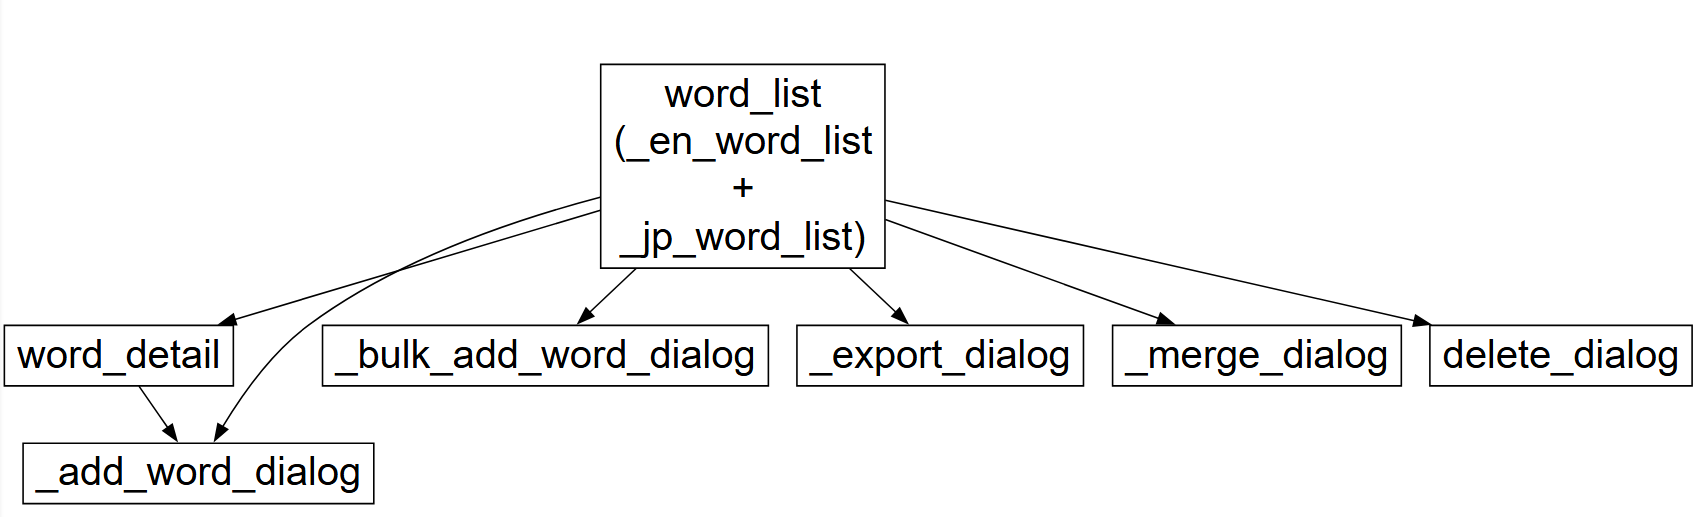
\includegraphics[width=1\textwidth]{images/impl/word_htmls.png}
  \caption{Szavakhoz tartozó HTML sablonok kapcsolatai}
  \label{fig:word-nav}
\end{figure}

\end{itemize}

\paragraph{Szótárak fő oldalai:}

\begin{itemize}
  \item \textbf{Szótárak listája (\texttt{dictionary\_list.html})}
  Ez a dictionary modul fő áttekintő felülete. Itt jelenik meg minden létrehozott szótár, típus (Word/Kanji) és nyelv szerint csoportosítva. A táblázat minden sorában láthatók a szótár neve, leírása és nyelve (zászló ikonként), elemei száma, aktuális statisztikái (új / jelenleg tanult / esedékes), valamint a szokásos műveletek: megnyitás, exportálás, egyesítés és törlés. A műveleti gombokhoz külön dialógusok tartoznak (\texttt{\_delete\_dialog.html}, \texttt{\_export\_dialog.html}, \texttt{\_merge\_dialog.html}, stb.), amelyek \texttt{include}-ként vannak betöltve. A kliensoldali logikát JavaScript metódusok segítségével valósítjuk meg. Ezekben történik az általános modálkezelés (megnyitás, bezárás, háttérre kattintás), validációs hibaüzenetek megjelenítése, a szerver által visszaadott hibák és az exportálási folyamat kezelése. A szótárakhoz kapcsolódó html file-ok felépítése a \ref{fig:dict-nav} ábrán látható.

  \item \textbf{Szótárak nézetei (\texttt{dictionary.html})}
  Ezek a \texttt{dictionary} objektumok egyedi nézetei, ahol a felhasználó áttekintheti az adott szótárhoz tartozó elemeket, statisztikákat és módosíthatja a beállításokat. A felső szekcióban megjelenő gomb segítségével tudjuk a beállítások modált megnyitni. A két statisztikai kártya a szótárhoz tartozó teljes elemszámot, illetve a napi új tanulási mennyiséget mutatja. A nézet két fő táblázatot tartalmaz, az egyik az elemeket és a hozzájuk tartozó szokásos statisztikát, valamint a szótárból való törlést biztosító gombot jeleníti meg, míg a másik a naponkénti tanulási statisztikákat. A további funkciókat két külön modál biztosítja: a szótár beállításai a \texttt{\_settings\_dialog.html} fájlból töltődnek be, míg a szabványos hibadialógus a \texttt{dashboard/includes/\_validation\_dialog.html} állományból érkezik. A kliensoldali logika a dictionary.js állományban található, amely kezeli a modálok megnyitását, a szerver-oldali hibaüzenetek megjelenítését és a beállítási űrlapok validációját, továbbá a törlési dialógusok működtetését.

  \item \textbf{Szótárak tanulási nézetei (\texttt{dictionary\_study.html})}
  Ez a sablon és a hozzá tartozó \texttt{study.js} modul valósítja meg a szótárakhoz kapcsolt tanulórendszert. A felület célja, hogy a felhasználó a kijelölt szótár elemeit a napi tanulási ciklus alapján, dinamikusan frissülő kártyák formájában tudja gyakorolni. A felület három fő szerkezeti egységre bontható, statisztikai panel, kártyanézet és válaszküldési logika. A felső komponens három értéket jelenít meg, az aznapi új tanulandó elemek számát, az éppen tanulási állapotban lévő tételeket, valamint az ismétlésre esedékes elemeket. Ezeket a kliens oldali \texttt{updateStats()} függvény a \texttt{/study-stats/} végpont hívásával frissíti, így a nyomon lehet követni a napi előrehaladást. 
    
  A tanulási folyamatot a kártyanézet vezérli, amely két részből áll. A kártya elején maga a szó vagy kanji jelenik meg, míg a hátulja tartalmazza az olvasatot, a jelentést, valamint további metaadatokat. A kártya hátoldalán kontextusgombok is helyet kapnak — „Kanji”, „Words”, „Sentences” — amelyek az adott elemhez kapcsolódó összefüggéseket (összetételek, származtatott szavak, mondatok) képesek megjeleníteni. Ezeket a szerver JSON-ként küldi vissza, míg megjelenítésük kliensoldali DOM-generálással történik.
    
  A tanulási ciklust a \texttt{loadStudyItems(), loadNextCard() és reloadIfNeeded()} függvények hajtják végre. A felhasználó először lekéri a napi tananyagot a \texttt{/study-data/} végponttal, majd sorban végigmegy a generált listán. Ha valamely válasz eredményeként egy elem visszakerül a gyakorlási sorba (Again válasz esetén), a rendszer újratölti a listát, így a tanulás folyamata dinamikusan alkalmazkodik a felhasználó teljesítményéhez.

  A négy válaszgomb mindegyike POST kérést küld az \texttt{/answer/} végponttal, megadva a kártya azonosítóját és a választott nehézségi szintet. A backend ennek alapján frissíti az adott elemet, majd a kliens automatikusan a következő kártyára lép. A felhasználói élményt billentyűparancsok is támogatják. A szóköz a válasz megjelenítését, 1–4 billentyűk a válaszok gyors kiválasztását segítik. Ha a napi tanulási anyag elfogyott, a rendszer egy külön állapotot jelenít meg, amely visszanavigálja a felhasználót a szótárak áttekintő oldalára.

\begin{figure}[H]
  \centering
  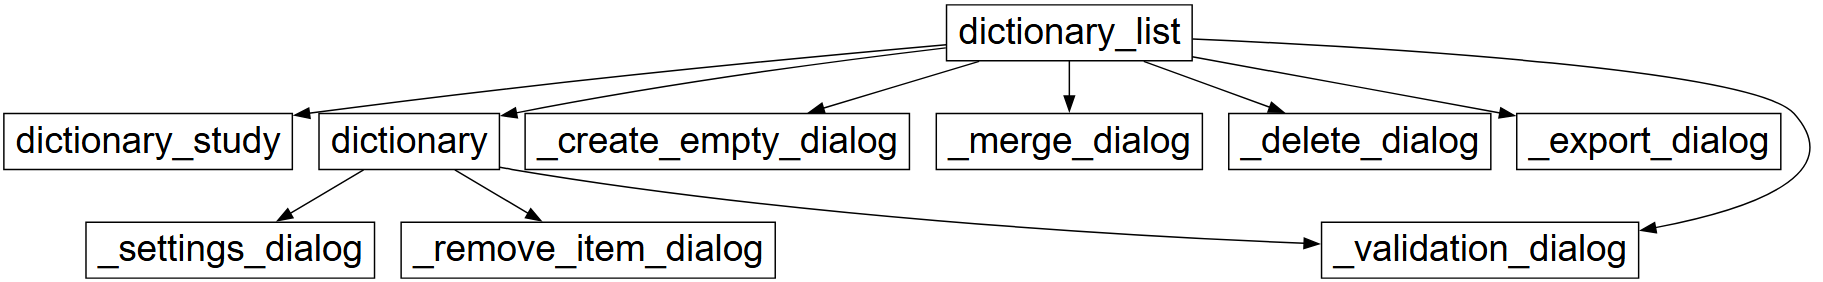
\includegraphics[width=1\textwidth]{images/impl/dict_htmls.png}
  \caption{Szótárakhoz tartozó HTML sablonok kapcsolatai}
  \label{fig:dict-nav}
\end{figure}

\end{itemize}

\section{Tesztelés}

A Django projektekben a tesztelést a modulonként automatikusan létrehozott \texttt{tests.py} fájlokban található beépített tesztkeretrendszert használó \textit{unittestek} végzik. Ezek lefedik a projekt legfontosabb területeit, itt kerül ellenőrzésre többek között a modellek, segédfüggvények, nézetek, API végpontok és a tanulási logika helyes működése. Az összes teszt egyszerre futtatható a \texttt{python manage.py test} paranccsal, de paraméterként meg lehet adni modulok nevét, a tesztosztályt vagy metódust is. A projekt és az eddigi dokumentáció mintáját követve, a tesztek applikációnként kerülnek bemutatásra.

\subsection{A \texttt{core} modul tesztjei}

A core modul a projekt alapját képező adatmodelleket tartalmazza. A tesztelés célja az adatbázis megszorítások (\texttt{unique, unique\_together, constraints}) és segédmetódusok (\texttt{get\_absolute\_url, meaning\_short}) megfelelő működésének ellenőrzése. Szintén itt vizsgáljuk meg, hogy a ManyToMany kapcsolatok megfelelően jönnek létre és lekérdezhetőek, valamint, hogy az adatok integritása megmarad-e hibás vagy duplikált bevitel esetén. A tesztek például ellenőrzik: 
\begin{itemize}
  \item \texttt{test\_word\_unique\_surface\_form}: Két azonos \texttt{surface\_form}-mal rendelkező szó létrehozása hibát okoz (\ref{src:word-unique-test}. kódrészlet)
  
  \item \texttt{test\_kanji\_meaning\_short\_truncation}: Egy kanji jelentésének rövidítése csak az első két jelentést adja vissza 
  
  \item \texttt{test\_word\_sentence\_many\_to\_many, test\_kanji\_word\_many\_to\_many}: A Word és Sentence, illetve Kanji és Word közötti kapcsolatok oda-vissza működését
    
  \item \texttt{test\_wordreference\_unique\_together}: A WordReference modellben ugyanazzal a (kanji, kana) párossal nem lehet duplikált rekordot létrehozni
\end{itemize}


\lstset{caption={A Word modell egyediségi szabály tesztje}, label=src:word-unique-test}
\begin{lstlisting}[language=Python]
def test_word_unique_surface_form(self):
    Word.objects.create(surface_form="unique_word")

    # Azonos surface_form -> errort kell dobnia
    with self.assertRaises(IntegrityError):
        Word.objects.create(surface_form="unique_word")
\end{lstlisting}

\subsection{A \texttt{dashboard} modul tesztjei}

A modul tesztjei fő feladata az, hogy megbizonyosodjunk arról, hogy a szűrési, keresési, statisztikai és listázási logika minden lehetséges bemenetre helyesen működjön, illetve a nézetek megfelelően kezeljék a felhasználói interakciókat és az adatbázis műveleteket. A tesztek sok helyen használnak segédfüggvényeket, HTTP kérések szimulációival. Többek között ellenőrzésre kerül, hogy:

\begin{itemize}
  \item \texttt{test\_apply\_search\_filter}: A keresési szűrő csak a megfelelő szavakat adja vissza (\ref{src:word-search-test} számú kódrészlet),
  \item \texttt{test\_apply\_date\_filters}: A dátum és esedékesség szerinti szűrés pontosan működik
  \item \texttt{test\_apply\_range\_filter}: A számtartomány szűrő helyesen választja ki a megfelelő rekordokat
  \item \texttt{test\_calculate\_text\_statistics} függvények: A szövegstatisztika számítás japán és angol szövegekre is helyes eredményt ad
  \item \texttt{test\_text\_merge\_execute}: Szövegek egyesítése sikeresen végrehajtható
  \item \texttt{test\_home\_view\_post\_valid}: A home nézet POST kérése érvényes adatokkal átirányítást eredményez
\end{itemize}

\lstset{caption={Keresési szűrő működésének tesztelése}, label=src:word-search-test}
\begin{lstlisting}[language=Python]
def test_apply_search_filter(self):
    word1 = Word.objects.create(surface_form="test", meaning="test meaning")
    word2 = Word.objects.create(surface_form="example", meaning="example meaning")

    queryset = Word.objects.all()
    filtered = apply_search_filter(queryset, "test", ["surface_form", "meaning"])
    self.assertEqual(filtered.count(), 1)
    self.assertEqual(filtered.first(), word1)
\end{lstlisting}

\subsection{A \texttt{processor} modul tesztjei}

A tesztelés célja annak ellenőrzése, hogy a japán és angol szövegek tokenizálása, mondatbontása, valamint a tartalom validálása minden esetben helyesen működik, továbbá a fájlbeolvasás és a nézetek is megfelelően kezelik a különböző bemeneteket és hibákat. Ezek fehér dobozos modultesztek, amelyek közvetlenül a segédfüggvényeket és a nézeteket hívják meg. A tesztek többek között ellenőrzik:

\begin{itemize}
  \item \texttt{test\_tokenize\_simple\_japanese\_text}: Egy egyszerű japán szöveg tokenizálásakor a megfelelő szavak, tulajdonnevek és karakterek felismerésre kerülnek
  \item \texttt{test\_takusan\_forms\_handling}: Egy szó amely több írott formában jelenik meg, egy objektumként jön létre, és mindkét olvasata megjelenik a lemmák között
  \item \texttt{test\_english\_pos\_filtering}: Az elemzett szöveg csak a szükséges szófajú szavakat menti el (\ref{src:english-tokenization} számú kódrészlet),
  \item \texttt{test\_japanese\_content\_validation}: A szöveg validációja hibát jelez üres tartalom esetén, de elfogadja a helyes japán vagy angol szöveget
  \item \texttt{test\_txt\_file\_extraction}: Fájlbeolvasás során sikeresen kinyeri a szöveget egy feltöltött .txt fájlból
\end{itemize}
  
\lstset{caption={Angol nyelvű tokenizálásnál szófaj alapú megkötések ellenőrzése}, label=src:english-tokenization}
\begin{lstlisting}[language=Python]
def test_english_pos_filtering(self):
    text = "The beautiful cat runs quickly."
    result = tokenize_english_text(text)
    lemmas = [lemma["surface_form"] for lemma in result["lemmas"]]
    
    # Noun, verb, adjective, adverb megvan, pronoun nem szerepel
    self.assertIn("cat", lemmas)
    self.assertIn("beautiful", lemmas)
    self.assertIn("run", lemmas)
    self.assertIn("quickly", lemmas)
    self.assertNotIn("the", lemmas)
\end{lstlisting}

\subsection{A \texttt{dictionary} modul tesztjei}

A modul tesztjei az itt definiált modellek, segédfüggvények, tanulási logika, API végpontok és nézetek helyes működését ellenőrzik. Példatesztek:

\begin{itemize}
    \item \texttt{test\_daily\_study\_stats\_unique\_together}: A  napi statisztikák (\texttt{DailyStudyStats}) egyediségét az adatbázis helyesen biztosítja
    
    \item \texttt{test\_remove\_item\_from\_dictionary, test\_dictionary\_items\_properties}: A szótárakhoz tartozó elemek helyesen lekérdezhetők, hozzáadhatók és eltávolíthatók
    
    \item \texttt{test\_dictionary\_merge\_execute, test\_merge\_different\_content\_types}: Szótár objektumok összevonása, és a hozzá tartozó hibakezelések
    
    \item \texttt{test\_create\_word\_dictionary\_from\_text, test\_create\_kanji...}: Egy szövegből helyesen jön létre szó- vagy kanji-szótár
    
    \item \texttt{test\_update\_item\_after\_answer\_new\_word, test\_update\_item\_after \_answer\_learning\_word, test\_four\_easy\_reviews\_interval\_growth}:  A tanulási rendszer logikája helyesen működik. Tanulási folyamatban lévő és ismétlődő szavak \texttt{status} paraméterének változása, intervallumok növekedése, statisztikák frissülése (\ref{src:srs-test} számú kódrészlet)
    
    \item \texttt{test\_dictionary\_study\_data\_api, test\_dictionary\_answer\_api}: Az API endpointok helyes JSON fájlokat adnak, és a tanulási folyamatot megfelelően frissítik
    
\end{itemize}

\lstset{caption={Szó frissülésének ellenőrzése a tanulói válaszok alapján}, label=src:srs-test}
\begin{lstlisting}[language=Python]
def test_new_word_again_then_easy(self):
    """new: Again (0) -> Easy (3) -> 4 nap"""
    word = Word.objects.create(surface_form="again_easy", status="new")
    self.dictionary.words.add(word)

    # 1: Again (0)
    update_item_after_answer(word, 0, self.dictionary)
    word.refresh_from_db()
    self.assertEqual(word.status, "learning")
    self.assertAlmostEqual(
        (word.next_review - timezone.now()).total_seconds(), 60, delta=5
    )
    self.assertLessEqual(word.ease_factor, 2.5)

    # 2: Easy (3)
    update_item_after_answer(word, 3, self.dictionary)
    word.refresh_from_db()
    self.assertEqual(word.status, "reviewing")
    # 4 nap mulva esedekes:
    self.assertAlmostEqual(
        (word.next_review.date() - date.today()).days, 4, delta=0
    )
\end{lstlisting}